% Options for packages loaded elsewhere
\PassOptionsToPackage{unicode}{hyperref}
\PassOptionsToPackage{hyphens}{url}
\PassOptionsToPackage{dvipsnames,svgnames,x11names}{xcolor}
%
\documentclass[
  letterpaper,
  DIV=11,
  numbers=noendperiod]{scrartcl}

\usepackage{amsmath,amssymb}
\usepackage{iftex}
\ifPDFTeX
  \usepackage[T1]{fontenc}
  \usepackage[utf8]{inputenc}
  \usepackage{textcomp} % provide euro and other symbols
\else % if luatex or xetex
  \usepackage{unicode-math}
  \defaultfontfeatures{Scale=MatchLowercase}
  \defaultfontfeatures[\rmfamily]{Ligatures=TeX,Scale=1}
\fi
\usepackage{lmodern}
\ifPDFTeX\else  
    % xetex/luatex font selection
\fi
% Use upquote if available, for straight quotes in verbatim environments
\IfFileExists{upquote.sty}{\usepackage{upquote}}{}
\IfFileExists{microtype.sty}{% use microtype if available
  \usepackage[]{microtype}
  \UseMicrotypeSet[protrusion]{basicmath} % disable protrusion for tt fonts
}{}
\makeatletter
\@ifundefined{KOMAClassName}{% if non-KOMA class
  \IfFileExists{parskip.sty}{%
    \usepackage{parskip}
  }{% else
    \setlength{\parindent}{0pt}
    \setlength{\parskip}{6pt plus 2pt minus 1pt}}
}{% if KOMA class
  \KOMAoptions{parskip=half}}
\makeatother
\usepackage{xcolor}
\setlength{\emergencystretch}{3em} % prevent overfull lines
\setcounter{secnumdepth}{-\maxdimen} % remove section numbering
% Make \paragraph and \subparagraph free-standing
\makeatletter
\ifx\paragraph\undefined\else
  \let\oldparagraph\paragraph
  \renewcommand{\paragraph}{
    \@ifstar
      \xxxParagraphStar
      \xxxParagraphNoStar
  }
  \newcommand{\xxxParagraphStar}[1]{\oldparagraph*{#1}\mbox{}}
  \newcommand{\xxxParagraphNoStar}[1]{\oldparagraph{#1}\mbox{}}
\fi
\ifx\subparagraph\undefined\else
  \let\oldsubparagraph\subparagraph
  \renewcommand{\subparagraph}{
    \@ifstar
      \xxxSubParagraphStar
      \xxxSubParagraphNoStar
  }
  \newcommand{\xxxSubParagraphStar}[1]{\oldsubparagraph*{#1}\mbox{}}
  \newcommand{\xxxSubParagraphNoStar}[1]{\oldsubparagraph{#1}\mbox{}}
\fi
\makeatother


\providecommand{\tightlist}{%
  \setlength{\itemsep}{0pt}\setlength{\parskip}{0pt}}\usepackage{longtable,booktabs,array}
\usepackage{calc} % for calculating minipage widths
% Correct order of tables after \paragraph or \subparagraph
\usepackage{etoolbox}
\makeatletter
\patchcmd\longtable{\par}{\if@noskipsec\mbox{}\fi\par}{}{}
\makeatother
% Allow footnotes in longtable head/foot
\IfFileExists{footnotehyper.sty}{\usepackage{footnotehyper}}{\usepackage{footnote}}
\makesavenoteenv{longtable}
\usepackage{graphicx}
\makeatletter
\def\maxwidth{\ifdim\Gin@nat@width>\linewidth\linewidth\else\Gin@nat@width\fi}
\def\maxheight{\ifdim\Gin@nat@height>\textheight\textheight\else\Gin@nat@height\fi}
\makeatother
% Scale images if necessary, so that they will not overflow the page
% margins by default, and it is still possible to overwrite the defaults
% using explicit options in \includegraphics[width, height, ...]{}
\setkeys{Gin}{width=\maxwidth,height=\maxheight,keepaspectratio}
% Set default figure placement to htbp
\makeatletter
\def\fps@figure{htbp}
\makeatother

\KOMAoption{captions}{tableheading}
\makeatletter
\@ifpackageloaded{caption}{}{\usepackage{caption}}
\AtBeginDocument{%
\ifdefined\contentsname
  \renewcommand*\contentsname{Table of contents}
\else
  \newcommand\contentsname{Table of contents}
\fi
\ifdefined\listfigurename
  \renewcommand*\listfigurename{List of Figures}
\else
  \newcommand\listfigurename{List of Figures}
\fi
\ifdefined\listtablename
  \renewcommand*\listtablename{List of Tables}
\else
  \newcommand\listtablename{List of Tables}
\fi
\ifdefined\figurename
  \renewcommand*\figurename{Figure}
\else
  \newcommand\figurename{Figure}
\fi
\ifdefined\tablename
  \renewcommand*\tablename{Table}
\else
  \newcommand\tablename{Table}
\fi
}
\@ifpackageloaded{float}{}{\usepackage{float}}
\floatstyle{ruled}
\@ifundefined{c@chapter}{\newfloat{codelisting}{h}{lop}}{\newfloat{codelisting}{h}{lop}[chapter]}
\floatname{codelisting}{Listing}
\newcommand*\listoflistings{\listof{codelisting}{List of Listings}}
\makeatother
\makeatletter
\makeatother
\makeatletter
\@ifpackageloaded{caption}{}{\usepackage{caption}}
\@ifpackageloaded{subcaption}{}{\usepackage{subcaption}}
\makeatother

\ifLuaTeX
  \usepackage{selnolig}  % disable illegal ligatures
\fi
\usepackage{bookmark}

\IfFileExists{xurl.sty}{\usepackage{xurl}}{} % add URL line breaks if available
\urlstyle{same} % disable monospaced font for URLs
\hypersetup{
  colorlinks=true,
  linkcolor={blue},
  filecolor={Maroon},
  citecolor={Blue},
  urlcolor={Blue},
  pdfcreator={LaTeX via pandoc}}


\author{}
\date{}

\begin{document}


\section{Carbon Nanotube and Graphene Field-Effect
Transistors}\label{sec-thin-film-transistors}

\subsection{Introduction}\label{introduction}

Out of a wide range of transducer options available for the creation of
compact, portable and highly-integrated biosensors, field-effect
transistors are among the most promising. Field-effect transistors
(FETs), initially proposed in the 1930s, consist of two conductive
electrodes on either side of a semiconducting channel, the `source' and
`drain' electrodes, alongside an isolated `gate' electrode which is
typically perpendicular to the channel. An applied electric field from
the gate electrode capacitively controls channel resistance, giving rise
to the label `field-effect'. By adjusting gate voltage, the flow of
charge carriers between source and drain can be varied over several
orders of magnitude. The ability of this simple structure to obtain a
large signal response from small changes in channel behaviour means
field-effect transistors can be used as high-quality amplifiers for
sensor applications {[}@Kauffman2008; @Petti2016; @Tran2016;
@Shkodra2021; @Yao2021{]}.

Carbon nanotube network and graphene field-effect transistors (CNT FETs
and GFETs) are both examples of a class of field-effect transistors
called thin-film transistors (TFTs). Thin-film transistors were first
developed in 1962 {[}@Weimer1962{]}, and are closely related to the
commonly-used metal oxide semiconductor field-effect transistor
(MOSFET). Unlike MOSFETs, thin-film transistors do not use the substrate
as the device channel. Instead, current passes through a semiconducting
film on the surface of the device; the films discussed here are graphene
and carbon nanotubes, two carbon-based low-dimension nanomaterials.
Since thin-film transistors do not require a conductive substrate, they
can be fabricated using light, flexible and stretchable substrates,
making them significantly more versatile than MOSFETs {[}@Kauffman2008;
@Cao2009; @Petti2016; @Shkodra2021{]}. Invisible conductive thin-films
such as metal oxides and carbon nanotube networks can also be used to
create transparent electronics {[}@Cao2009{]}. While the principle of
modulating current with a gate electrode is shared by the MOSFET and
TFT, the underlying physics behind the transistor behaviour differs
between the two. The MOSFET is turned on by the change in carrier
behaviour when switching from a depletion to an inversion mode, while
this is not the case for a TFT {[}@Petti2016{]}. Details of graphene and
carbon nanotube TFT switching behaviours can be found in the subsequent
sections.

\subsection{Thin-Film Field-Effect Transistors}\label{sec-general-FETs}

\subsubsection{Structure and Gating}\label{sec-gating}

\begin{figure}

\begin{minipage}{0.03\linewidth}
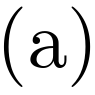
\includegraphics{figures/(a).png}\end{minipage}%
%
\begin{minipage}{0.01\linewidth}
~\end{minipage}%
%
\begin{minipage}{0.45\linewidth}
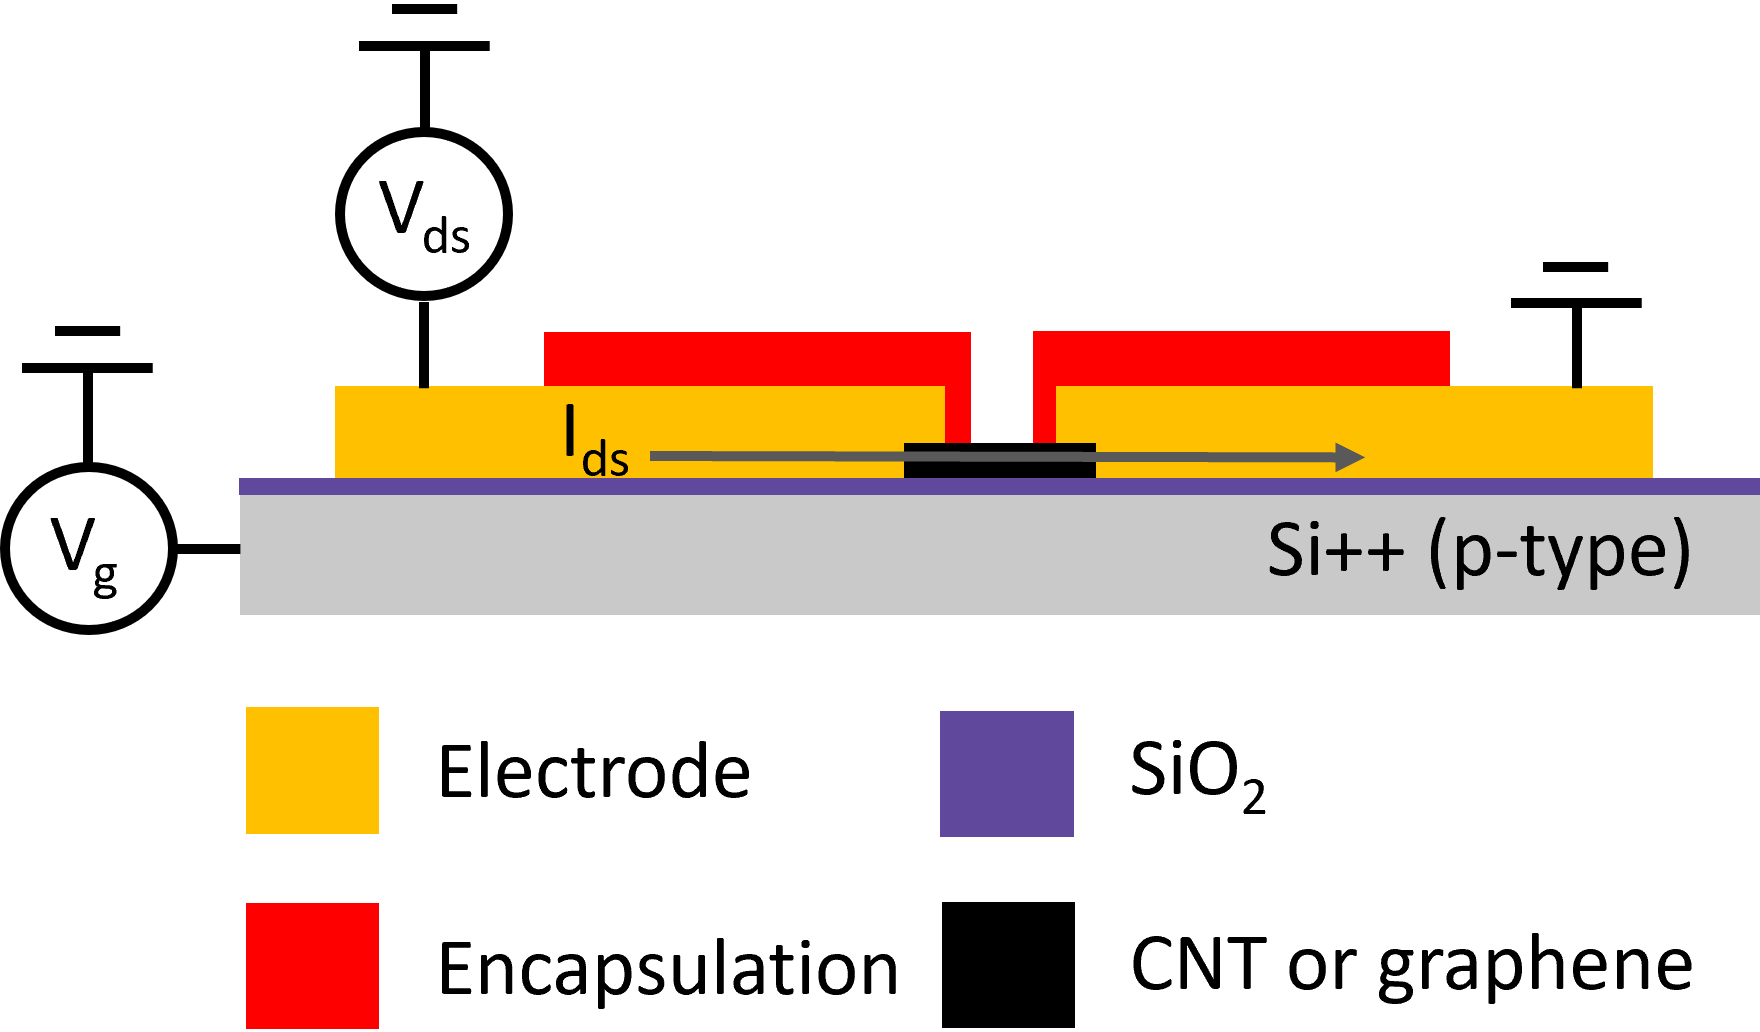
\includegraphics{figures/ch2/back-gate-schematic.png}\end{minipage}%
%
\begin{minipage}{0.01\linewidth}
~\end{minipage}%
%
\begin{minipage}{0.03\linewidth}
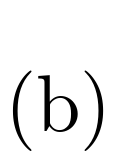
\includegraphics{figures/(b).png}\end{minipage}%
%
\begin{minipage}{0.01\linewidth}
~\end{minipage}%
%
\begin{minipage}{0.45\linewidth}
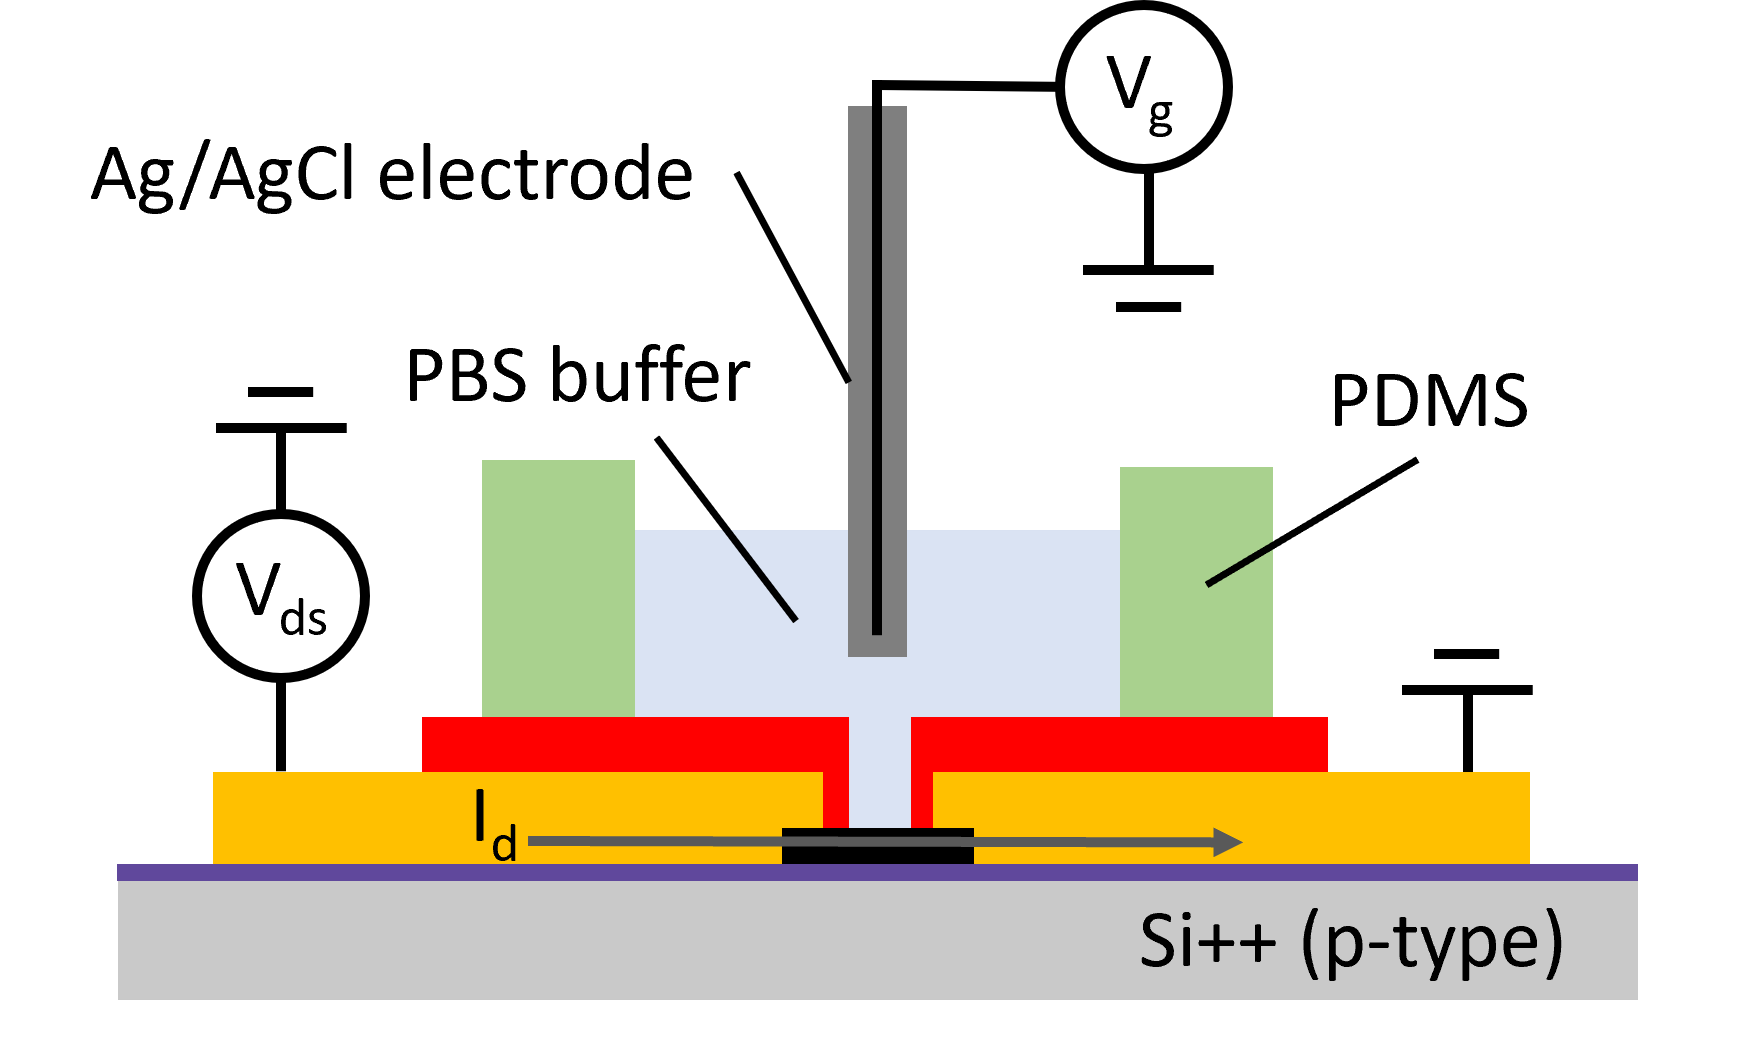
\includegraphics{figures/ch2/liquid-gate-schematic.png}\end{minipage}%
%
\begin{minipage}{0.01\linewidth}
~\end{minipage}%

\caption{\label{fig-gating-schematics}Schematics (not to scale) showing
the side-view cross-section of a thin-film field-effect transistor in
both the (a) back-gated and (b) liquid-gated configuration. Here, a
graphene monolayer or a carbon nanotube network is used as the
transistor thin-film. The drain electrode is the gold contact on the
left side of each figure, while the source electrode is the gold contact
on the right.}

\end{figure}%

Two basic configurations of the thin-film transistor are the back-gated
field-effect transistor and the liquid-gated (or electrolyte-gated)
transistor. The relatively simple back-gated configuration, shown in
Figure~\ref{fig-gating-schematics} (a), uses the degenerately doped Si
substrate as the gate. The channel is isolated from the gate with a thin
SiO\(_2\) layer. A liquid-gated device, shown in
Figure~\ref{fig-gating-schematics} (b), is used for sensitive
liquid-phase analyte detection. A submerged Ag/AgCl reference electrode
is generally used as a top-gate in this configuration. The channel is
isolated from the gate by the bulk of an electrolyte solution, which can
be restricted to the channel area using a hydrophobic
polydimethylsiloxane microchamber or `PDMS well'. The electrolyte used
is typically the biofriendly phosphate-buffered saline (PBS), but other
aqueous salt solutions, polymers and ion-gels have also been used
{[}@Avouris2007; @Shkodra2021; @Tran2016; @Li2023{]}. Transistor
operation is controlled by a `drain' bias \(V_{ds}\), placed between the
drain and source electrodes, and a `gate' bias \(V_g\), placed between
the gate and source electrodes. Gate capacitance determines the
influence of \(V_g\) on drain-source current \(I_d\). In general, gate
capacitance is a series combination of geometric capacitance, \(C_{G}\),
and the quantum capacitance of the channel nanomaterial, \(C_{Q}\)
{[}@Avouris2007; @Cao2009; @Heller2009a; @Tran2016; @Kireev2017;
@Li2023{]}.

\paragraph*{Liquid-Gating and Debye
Length}\label{liquid-gating-and-debye-length}
\addcontentsline{toc}{paragraph}{Liquid-Gating and Debye Length}

Understanding the ionic behaviour of the gate electrolyte used in a
liquid-gated device setup gives insight into the gating and sensing
behaviour of the setup. When a voltage is applied at the liquid-gate,
the charged ions in solution move to form two electric double layers,
one at the interface between the electrolyte and gate electrode, and one
at the interface between electrolyte and semiconducting channel, as
shown in Figure~\ref{fig-Debye-length}. The gate capacitance is a series
combination of the capacitance of each EDL in series with quantum
capacitance \(C_{Q}\) {[}@Heller2010; @Kireev2017; @Shkodra2021{]}. The
Gouy-Chapman-Stern model splits the EDL into two distinct regions, the
first being a compact layer of ions, the Stern layer, and the second
being a more diffuse layer, the Gouy-Chapman layer {[}@Tiwari2022{]}.
The surface potential of the solid-electrolyte interface exponentially
decreases across the diffuse region of the double-layer; the
characteristic length of this potential screening is known as Debye
length, \(\lambda_D\). The typical electrolyte Debye length is on a
nanometer scale, therefore the bulk electrolyte acts as an insulator,
similar to the SiO\(_2\) dielectric in the back-gated configuration. The
Stern layer capacitance is inversely proportional to the Debye length,
and therefore decreased \(\lambda_D\) corresponds to increased gate
capacitance {[}@Heller2010; @Ohno2015; @Shkodra2021; @Yao2021{]}.

\begin{figure}

\centering{

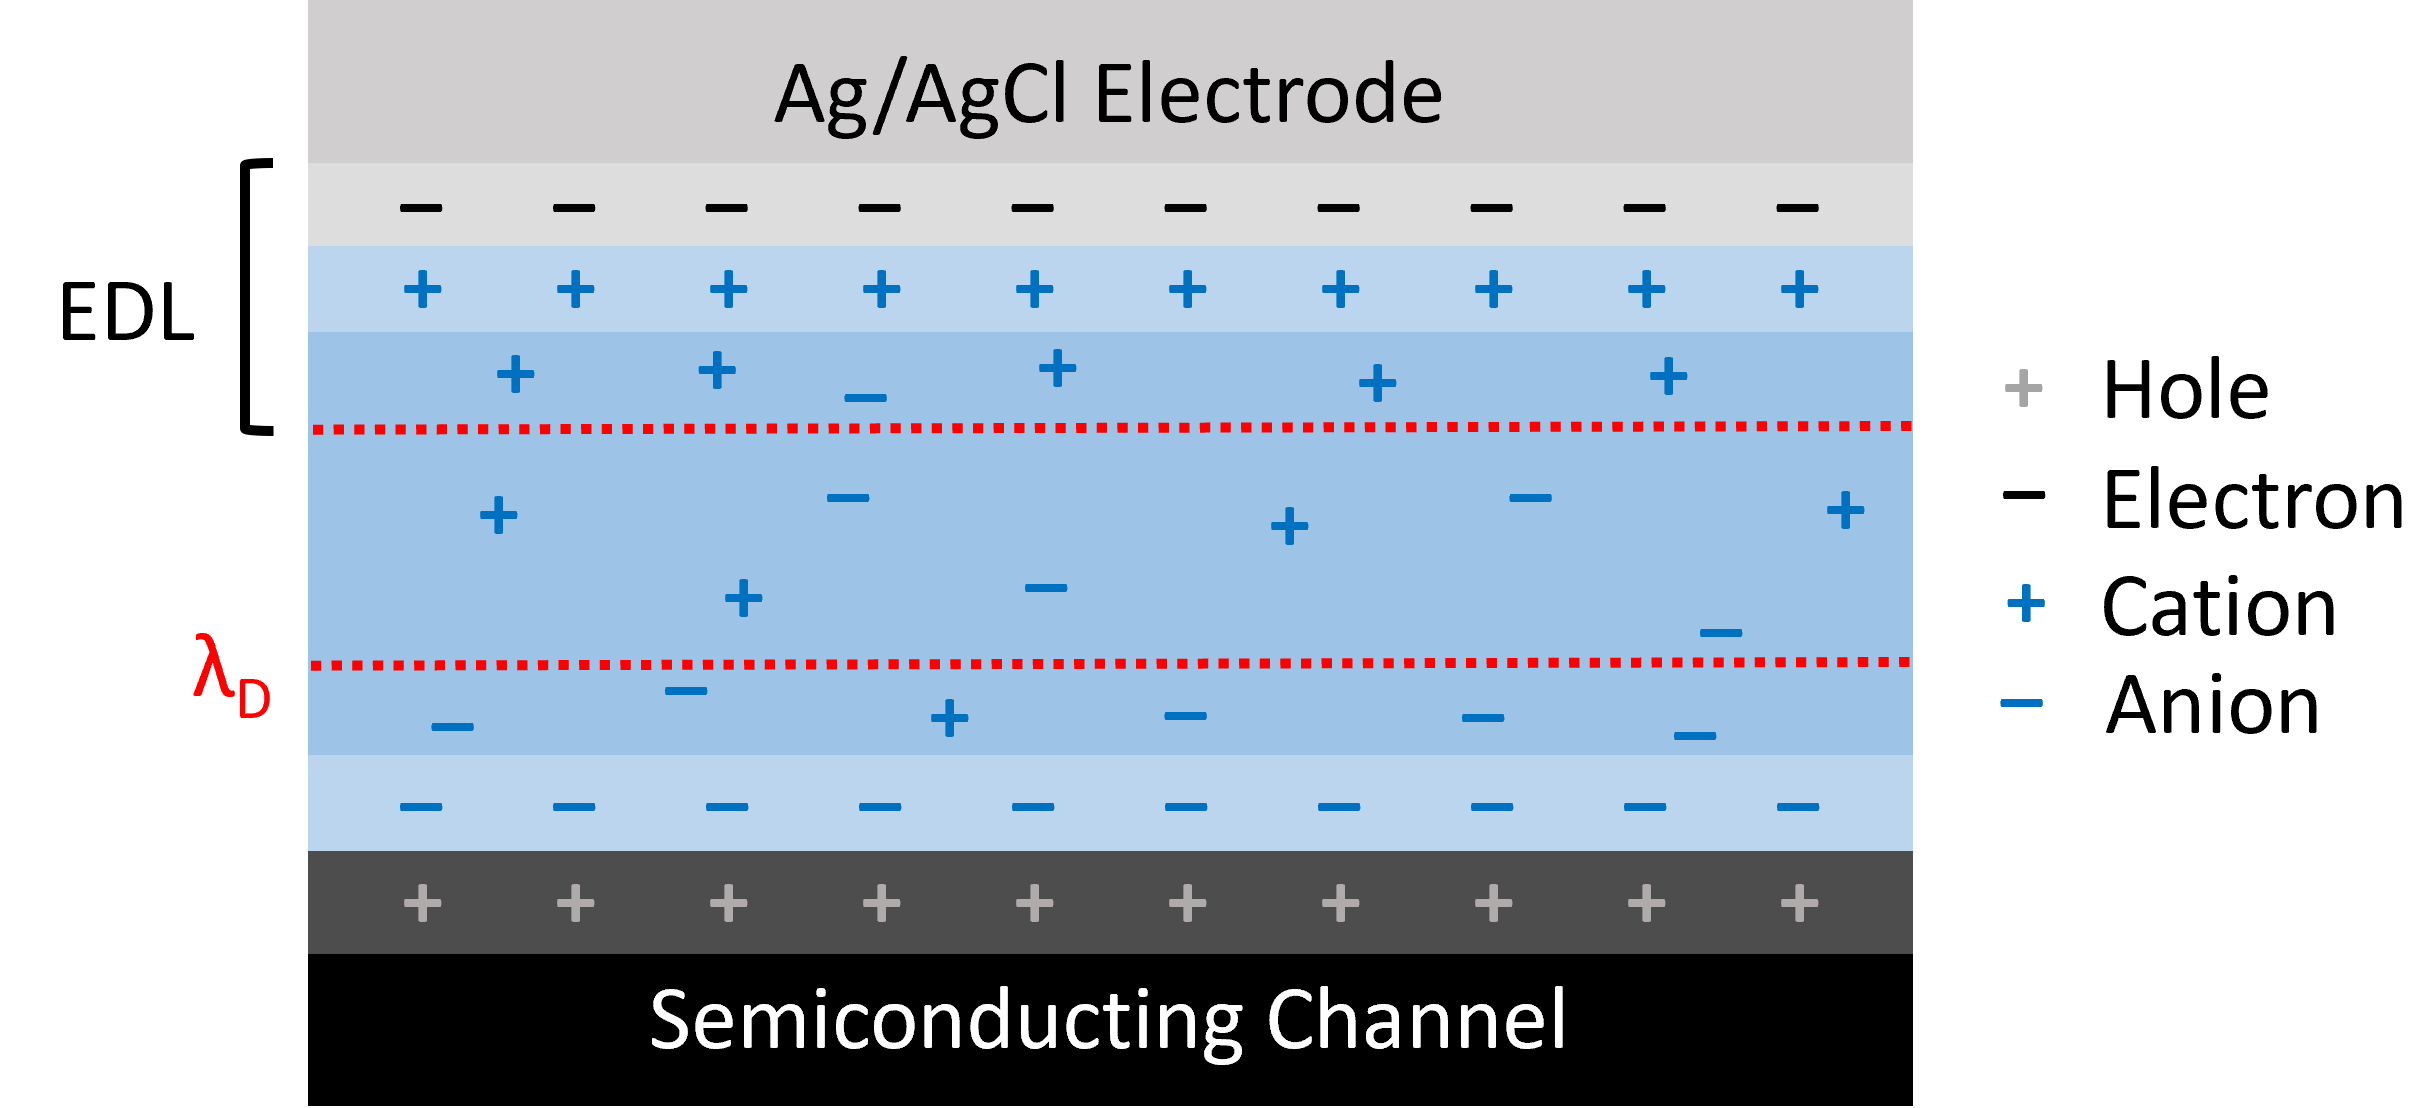
\includegraphics[width=0.7\textwidth,height=\textheight]{figures/ch2/Debye-length-schematic-alt.png}

}

\caption{\label{fig-Debye-length}A diagram of the formation of an
electric double layer (EDL) under an applied voltage between source and
liquid-gate electrodes, with a \(p\)-type semiconductor used for the
channel thin-film. Electric double layers are present at both the
gate-electrolyte interface and semiconductor-electrolyte interface.
Adapted from {[}@Ohno2015; @Shkodra2021; @Tiwari2022{]}.}

\end{figure}%

The equation for Debye length \(\lambda_D\) in an electrolyte solution
is given by Equation~\ref{eq-debye-length}.

\begin{equation}\phantomsection\label{eq-debye-length}{
\lambda_D = \sqrt{\frac{\epsilon_0\epsilon_rk_bT}{2N_Aq^2I}}
}\end{equation}

Here, \(\epsilon_0\) is vacuum permittivity, \(\epsilon_r\) is the
relative permittivity of the electrolyte, \(\k_B\) is the Boltzmann
constant, \(T\) is absolute temperature in K, \(N_A\) is the Avogadro
number, \(q\) is the elementary charge and \(I\) is ionic strength in
mmol L\(^{-1}\). When temperature is kept constant, \(\lambda_D\) only
depends on the ionic strength of the electrolyte and not on any
attributes of the gate electrode or channel {[}@Stern2007;
@Shkodra2021{]}. Successive dilutions of a particular electrolyte will
increase the Debye length: for \(1 \times\) PBS, \(\lambda_D\) is
\(\sim\) 1 nm, for \(0.1 \times\) PBS, \(\lambda_D\) is \(\sim\) 2 nm,
for \(0.01 \times\) PBS \(\lambda_D\) is \(\sim\) 8 nm and so on. This
means gate capacitance is directly dependent on the electrolyte used and
its concentration {[}@Kireev2017; @Shkodra2021{]}. A \(1 \times\) PBS
electrolyte gives a gate capacitance several orders of magnitude larger
than that of a SiO\(_2\) back-gate. A larger capacitance significantly
increases the effect of electrostatic gating on the channel current,
often described as increased electrostatic coupling between gate and
channel. A liquid-gated device with low Debye length will therefore be
highly sensitive to electrostatic changes across a small voltage range
{[}@Heller2010; @Ohno2015; @Kireev2017; @Yao2021{]}.

However, a decreased Debye length also has disadvantages for sensing.
Electrostatic potentials outside of the electrolyte-channel electrical
double layer are effectively screened from the channel. Electrical
double layers will also form around charged receptors within the
solution. The combined screening effect means signals due to potential
changes in charged biomolecules within the bulk electrolyte will have no
effect on gating of the channel, and therefore no effect on \(I_d\).
Interactions between the analyte and any receptor element must therefore
occur within the Debye length, and so a tradeoff exists between channel
sensitivity and the size of the sensitive region above the channel. Many
medium or large proteins will require a relatively dilute electrolyte
for analyte capture to be detected by the channel, which may not reflect
the intended environment for biosensor application {[}@Stern2007;
@Piccinini2018; @Shkodra2021{]}. Other approaches to increasing Debye
length without reducing device sensitivity have therefore also been
trialled. One approach involves attaching a layer of polyethylene glycol
polymer (PEG) to the channel, limiting the approach of counterions. This
increases Debye length at the electrolyte-channel interface while
preserving the capacitance of the electrolyte-gate interface, keeping
device sensitivity relatively high {[}@Gao2016; @Filipiak2018;
@Kesler2020; @Albarghouthi2022{]}.

\subsubsection{Electrical
Characterisation}\label{electrical-characterisation}

\begin{figure}

\centering{

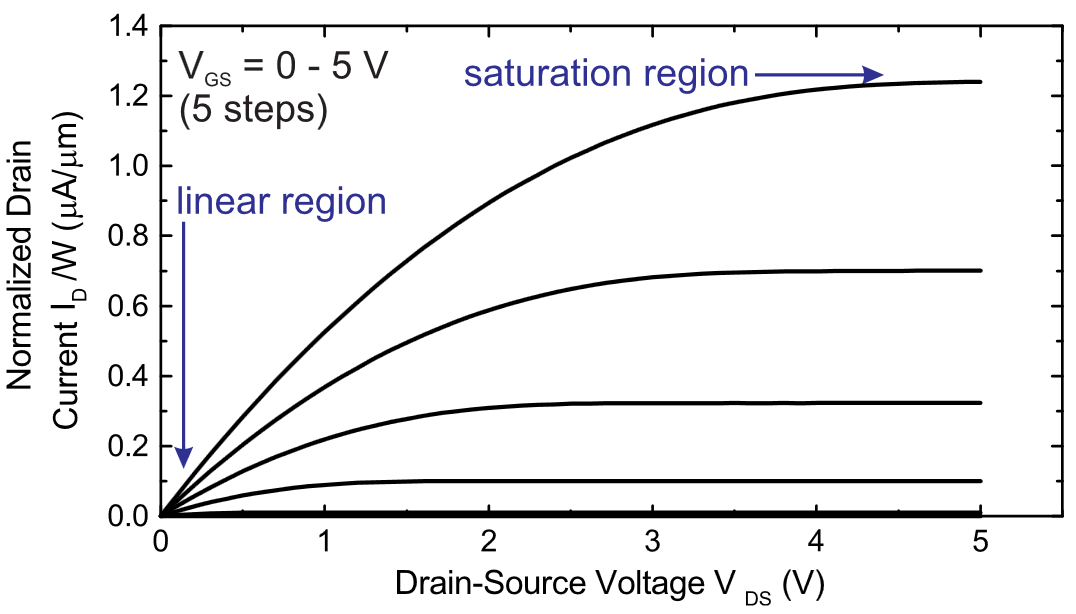
\includegraphics[width=0.65\textwidth,height=\textheight]{figures/ch2/linear_region_edit.png}

}

\caption{\label{fig-linear-region}The linear and saturation operation
regimes of an \(n\)-type metal oxide semiconductor TFT, \(V_{t} \sim 0\)
V. Current has been normalised with respect to channel width (W).
Reproduced with permission from {[}@Petti2016{]}.}

\end{figure}%

The current-voltage plots of a given transistor are known as its
`characteristic curves'. The I-V curve of \(I_d\) against \(V_{ds}\) at
constant \(V_g\) is known as the `source-drain' or `output'
characteristic curve, while \(I_d\) against \(V_g\) at constant
\(V_{ds}\) is known as the `transfer' characteristic curve at that
source-drain voltage {[}@Kauffman2008; @Petti2016; @Shkodra2021{]}.
Applying a gate voltage \(V_g\) to the gate of an thin-film transistor
influences the amount and type of available charge carriers for
conduction {[}@Avouris2007; @Tran2016; @Heller2009a{]}. In an ambipolar
transistor, a highly negative \(V_g\) will give rise to hole conduction,
and a highly positive \(V_g\) will give rise to electron conduction
{[}@Avouris2007; @Yao2021; @Li2023{]}. The minimum \(V_g\) required to
turn the flow of current in a thin-film transistor `on' is referred to
as the threshold voltage \(V_t\) {[}@Petti2016; @Shkodra2021;
@Li2023{]}. Threshold voltage is discussed in more detail in
Section~\ref{sec-electrical-characterisation-CNT}. When
\(|V_{ds}| < |V_g| - |V_t|\) while \(|V_g|>|V_t|\), the device is in the
linear regime. Here, \(V_{ds}\) is directly proportional to \(I_{d}\),
similar to an Ohmic resistor. When \(|V_{ds}| > |V_g| - |V_t|\) and
\(|V_g|>|V_t|\), the device is in the saturation regime, where the
relationship between \(V_{ds}\) and \(I_{d}\) becomes non-linear
{[}@Petti2016; @Shkodra2021; @Li2023{]}.

\begin{figure}

\begin{minipage}{0.03\linewidth}
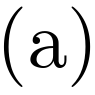
\includegraphics{figures/(a).png}\end{minipage}%
%
\begin{minipage}{0.01\linewidth}
~\end{minipage}%
%
\begin{minipage}{0.45\linewidth}
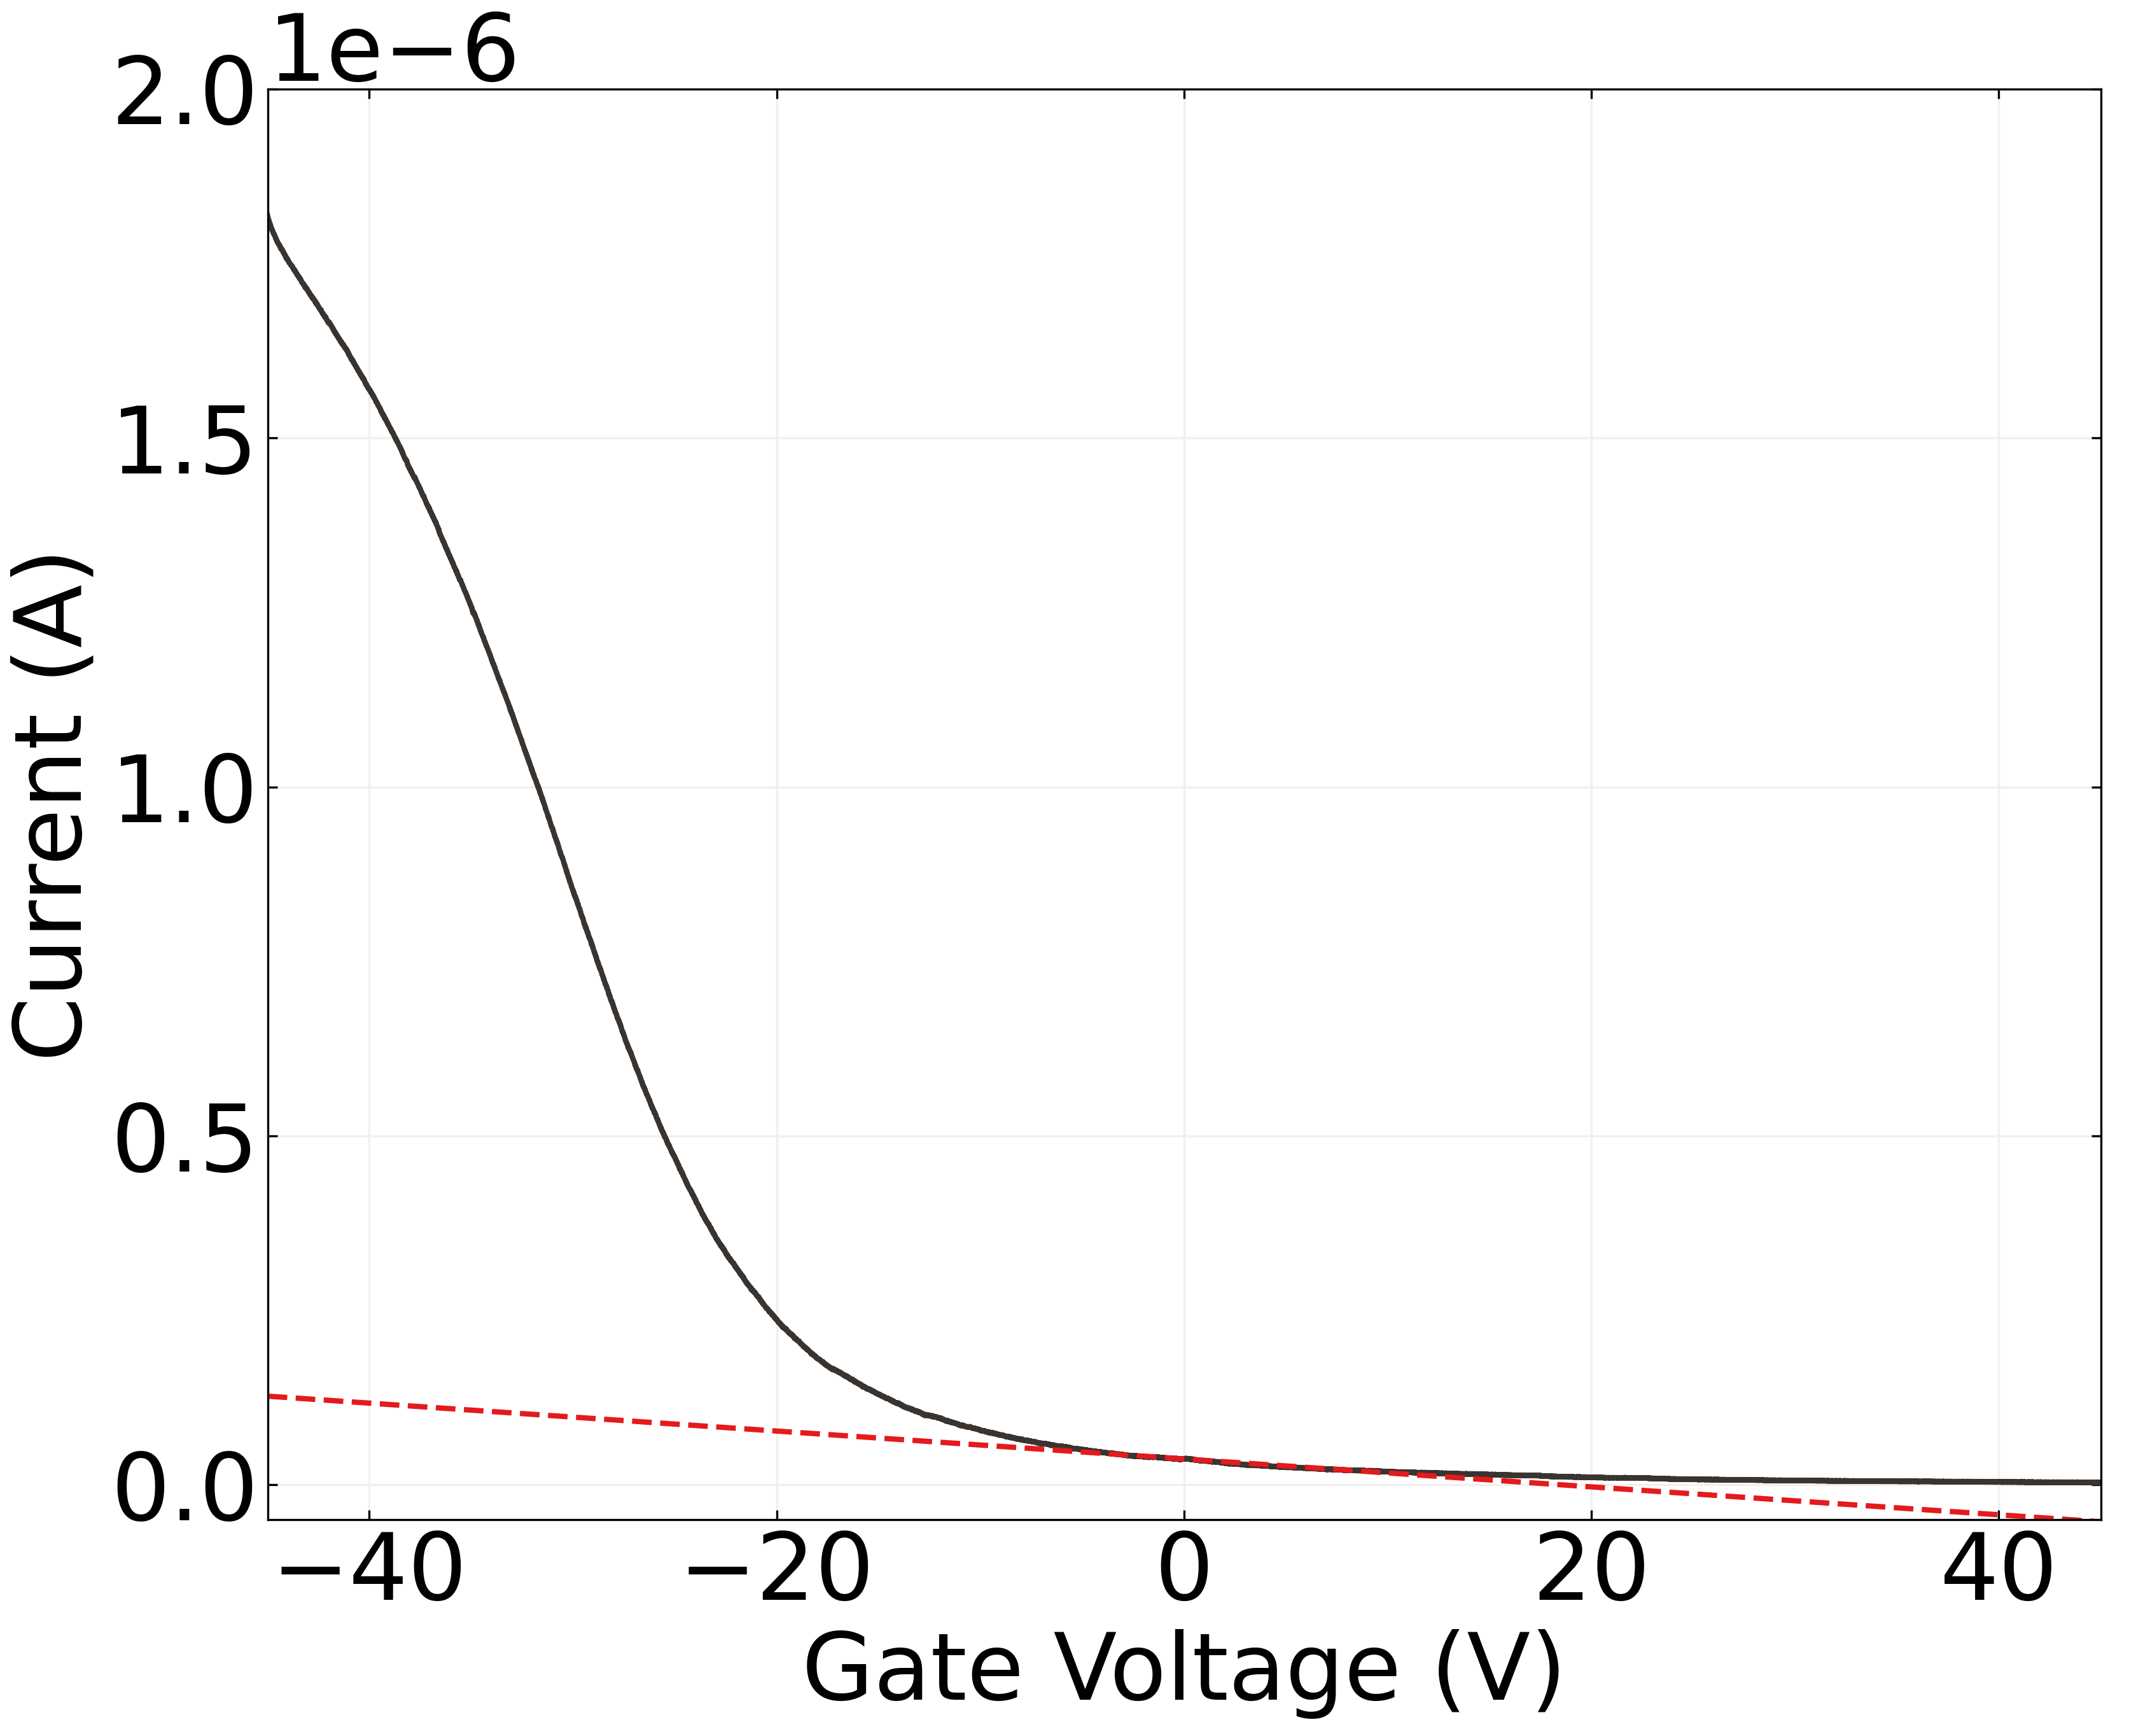
\includegraphics{figures/ch2/Q5C10ch8transconductance.png}\end{minipage}%
%
\begin{minipage}{0.01\linewidth}
~\end{minipage}%
%
\begin{minipage}{0.03\linewidth}
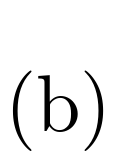
\includegraphics{figures/(b).png}\end{minipage}%
%
\begin{minipage}{0.01\linewidth}
~\end{minipage}%
%
\begin{minipage}{0.45\linewidth}
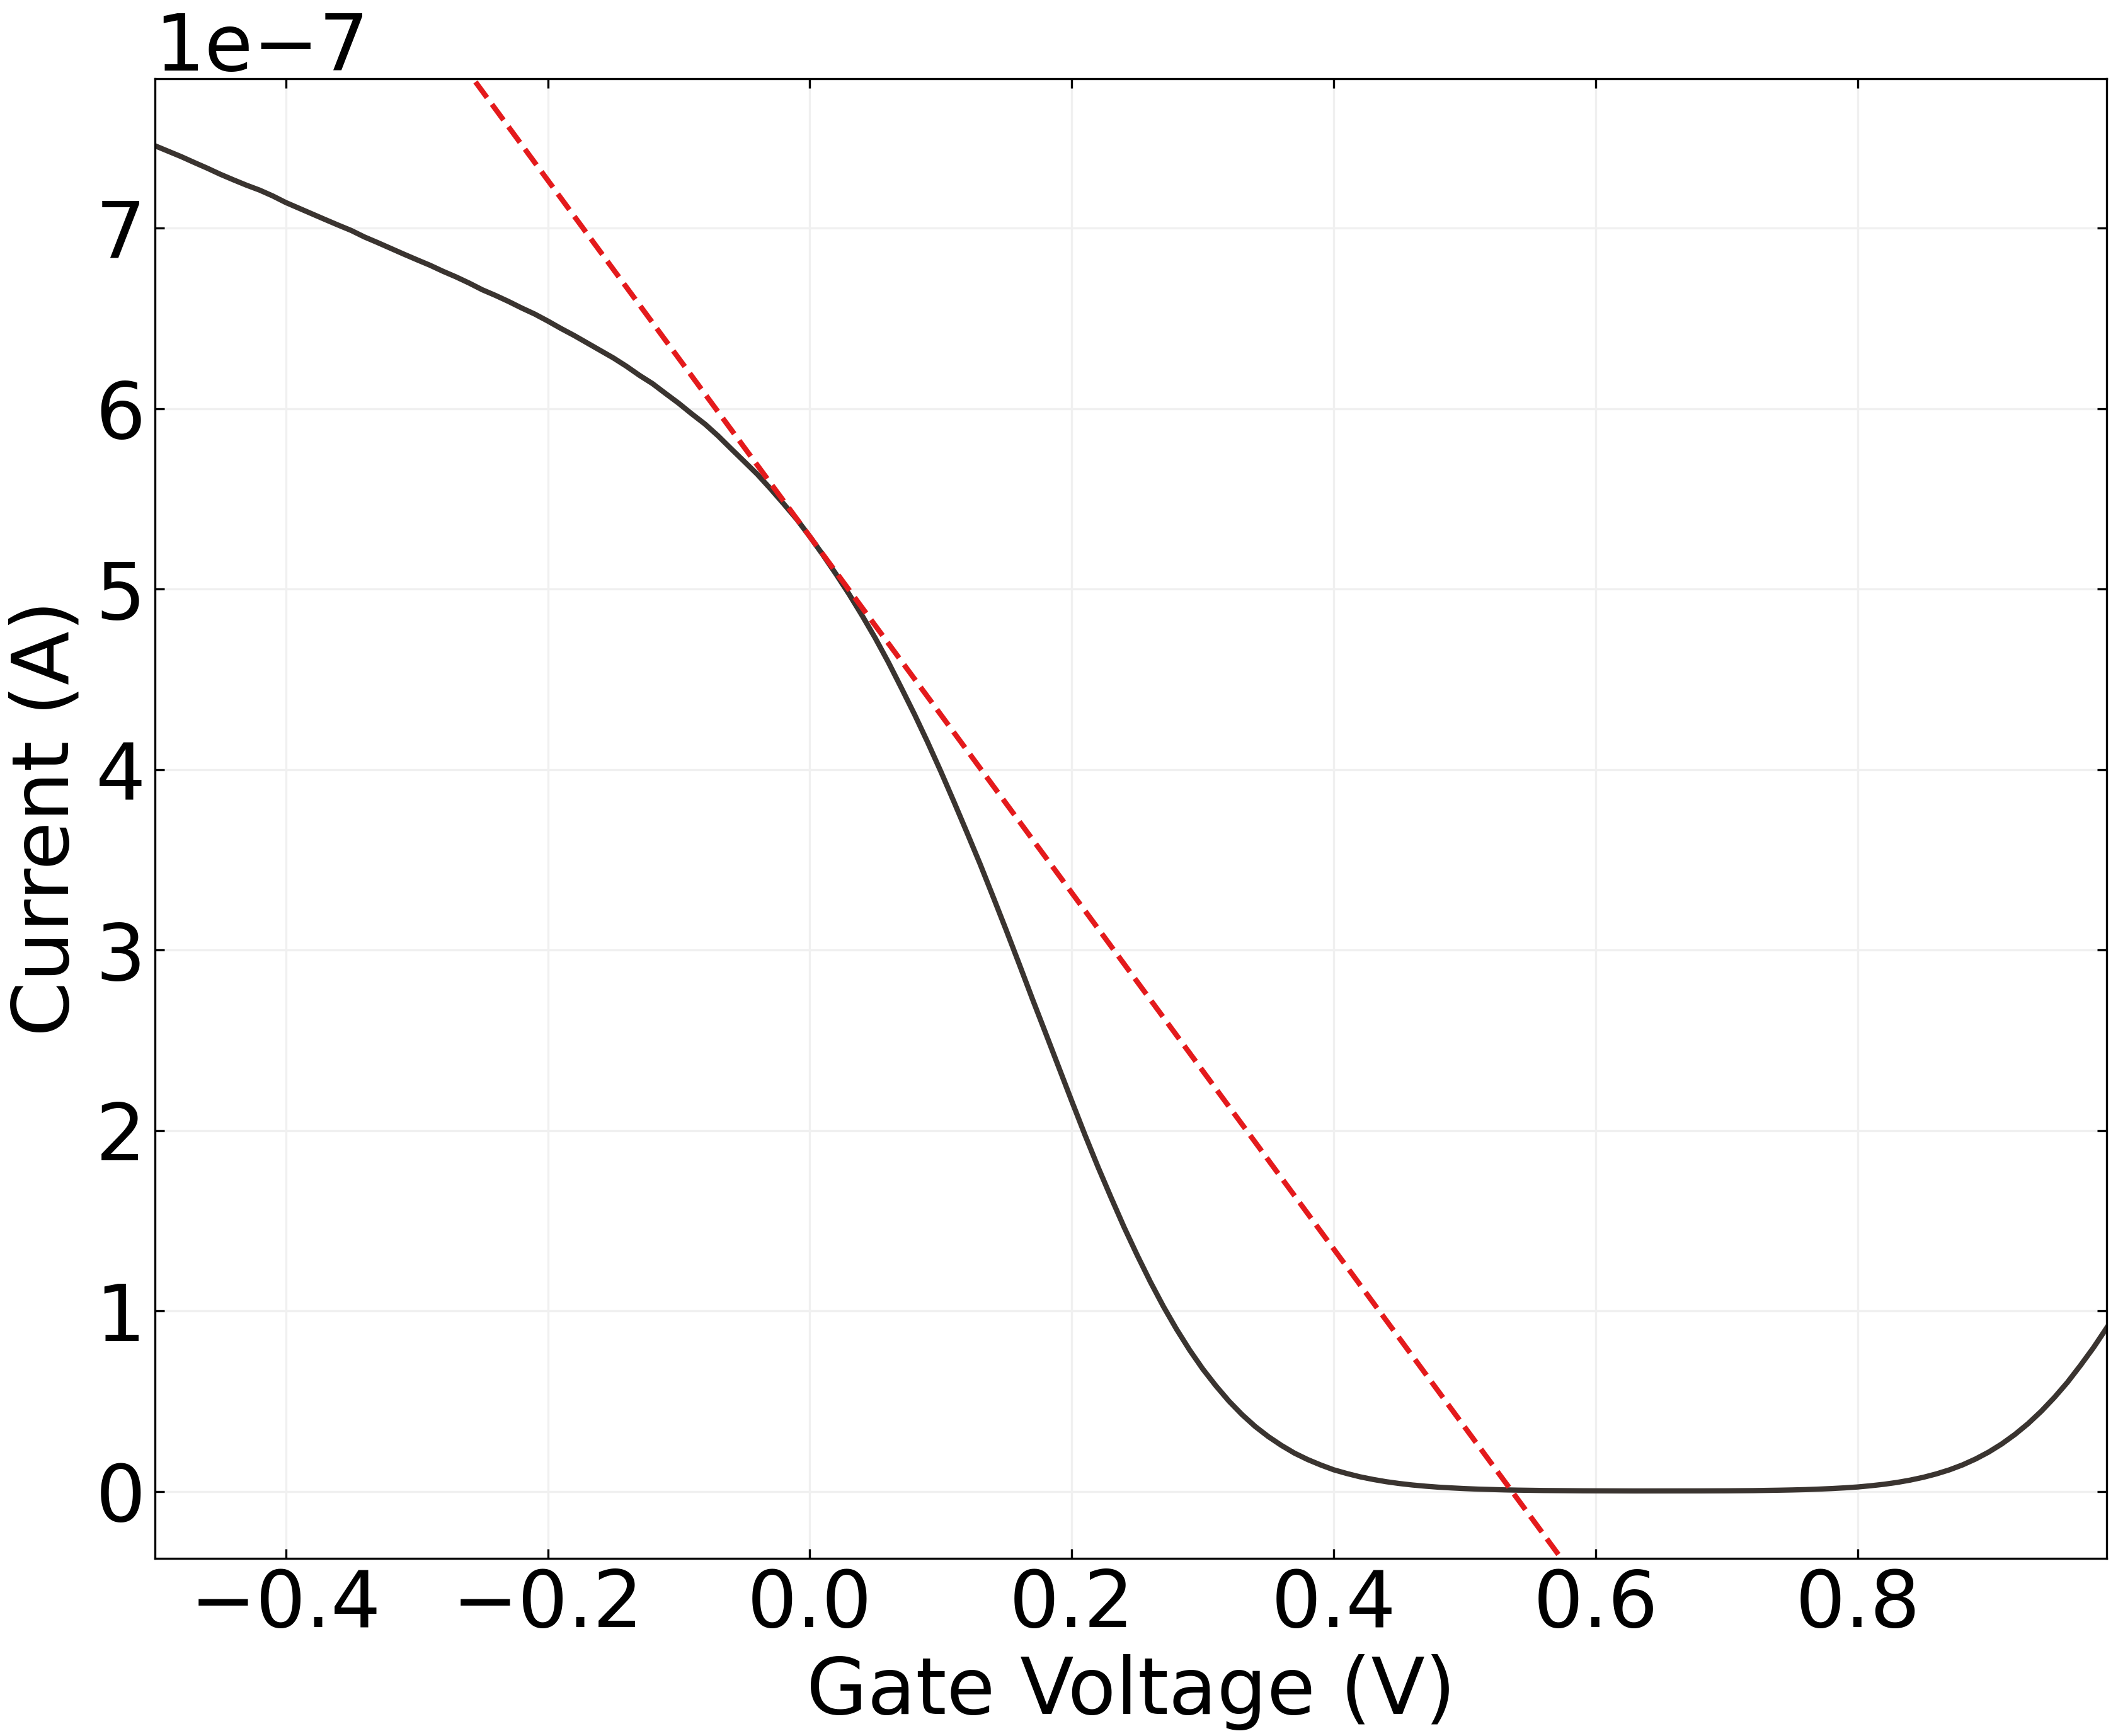
\includegraphics{figures/ch2/NTQ31C5ch1transconductance.png}\end{minipage}%
%
\begin{minipage}{0.01\linewidth}
~\end{minipage}%
\newline
\begin{minipage}{0.03\linewidth}
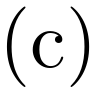
\includegraphics{figures/(c).png}\end{minipage}%
%
\begin{minipage}{0.01\linewidth}
~\end{minipage}%
%
\begin{minipage}{0.45\linewidth}
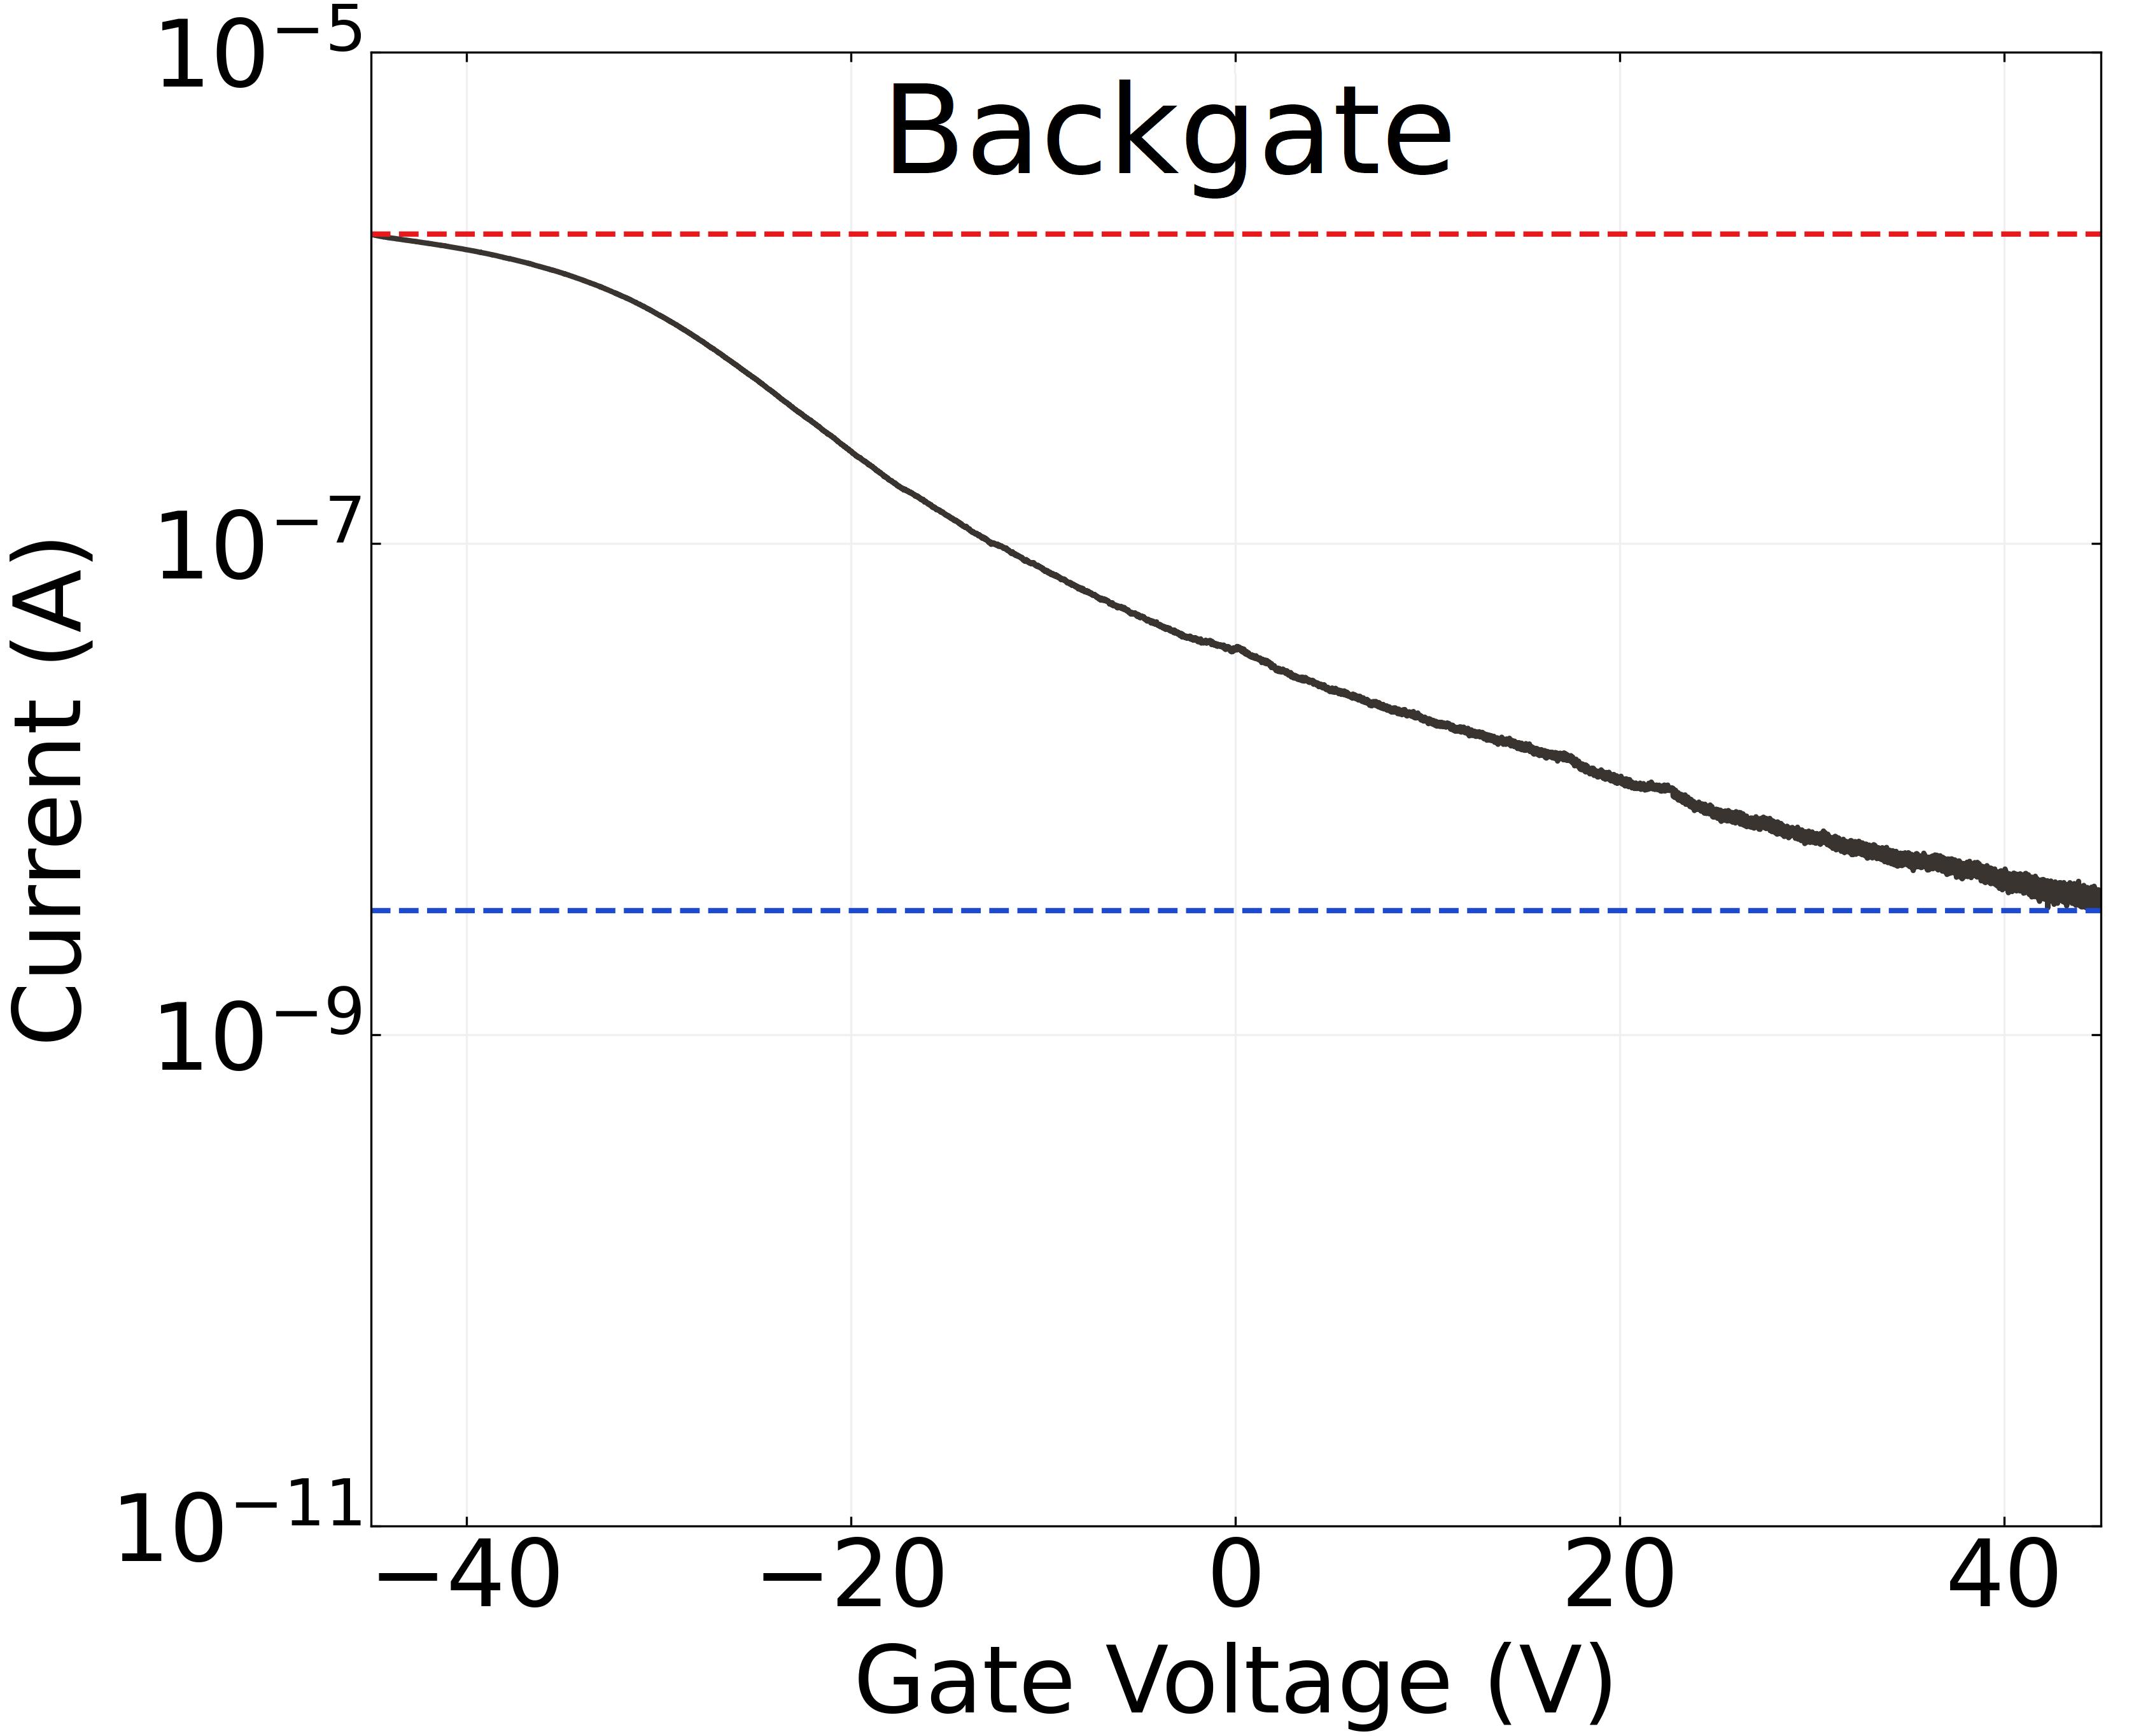
\includegraphics{figures/ch2/Q5C10ch8on_off_current.png}\end{minipage}%
%
\begin{minipage}{0.01\linewidth}
~\end{minipage}%
%
\begin{minipage}{0.03\linewidth}
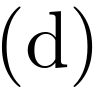
\includegraphics{figures/(d).png}\end{minipage}%
%
\begin{minipage}{0.01\linewidth}
~\end{minipage}%
%
\begin{minipage}{0.45\linewidth}
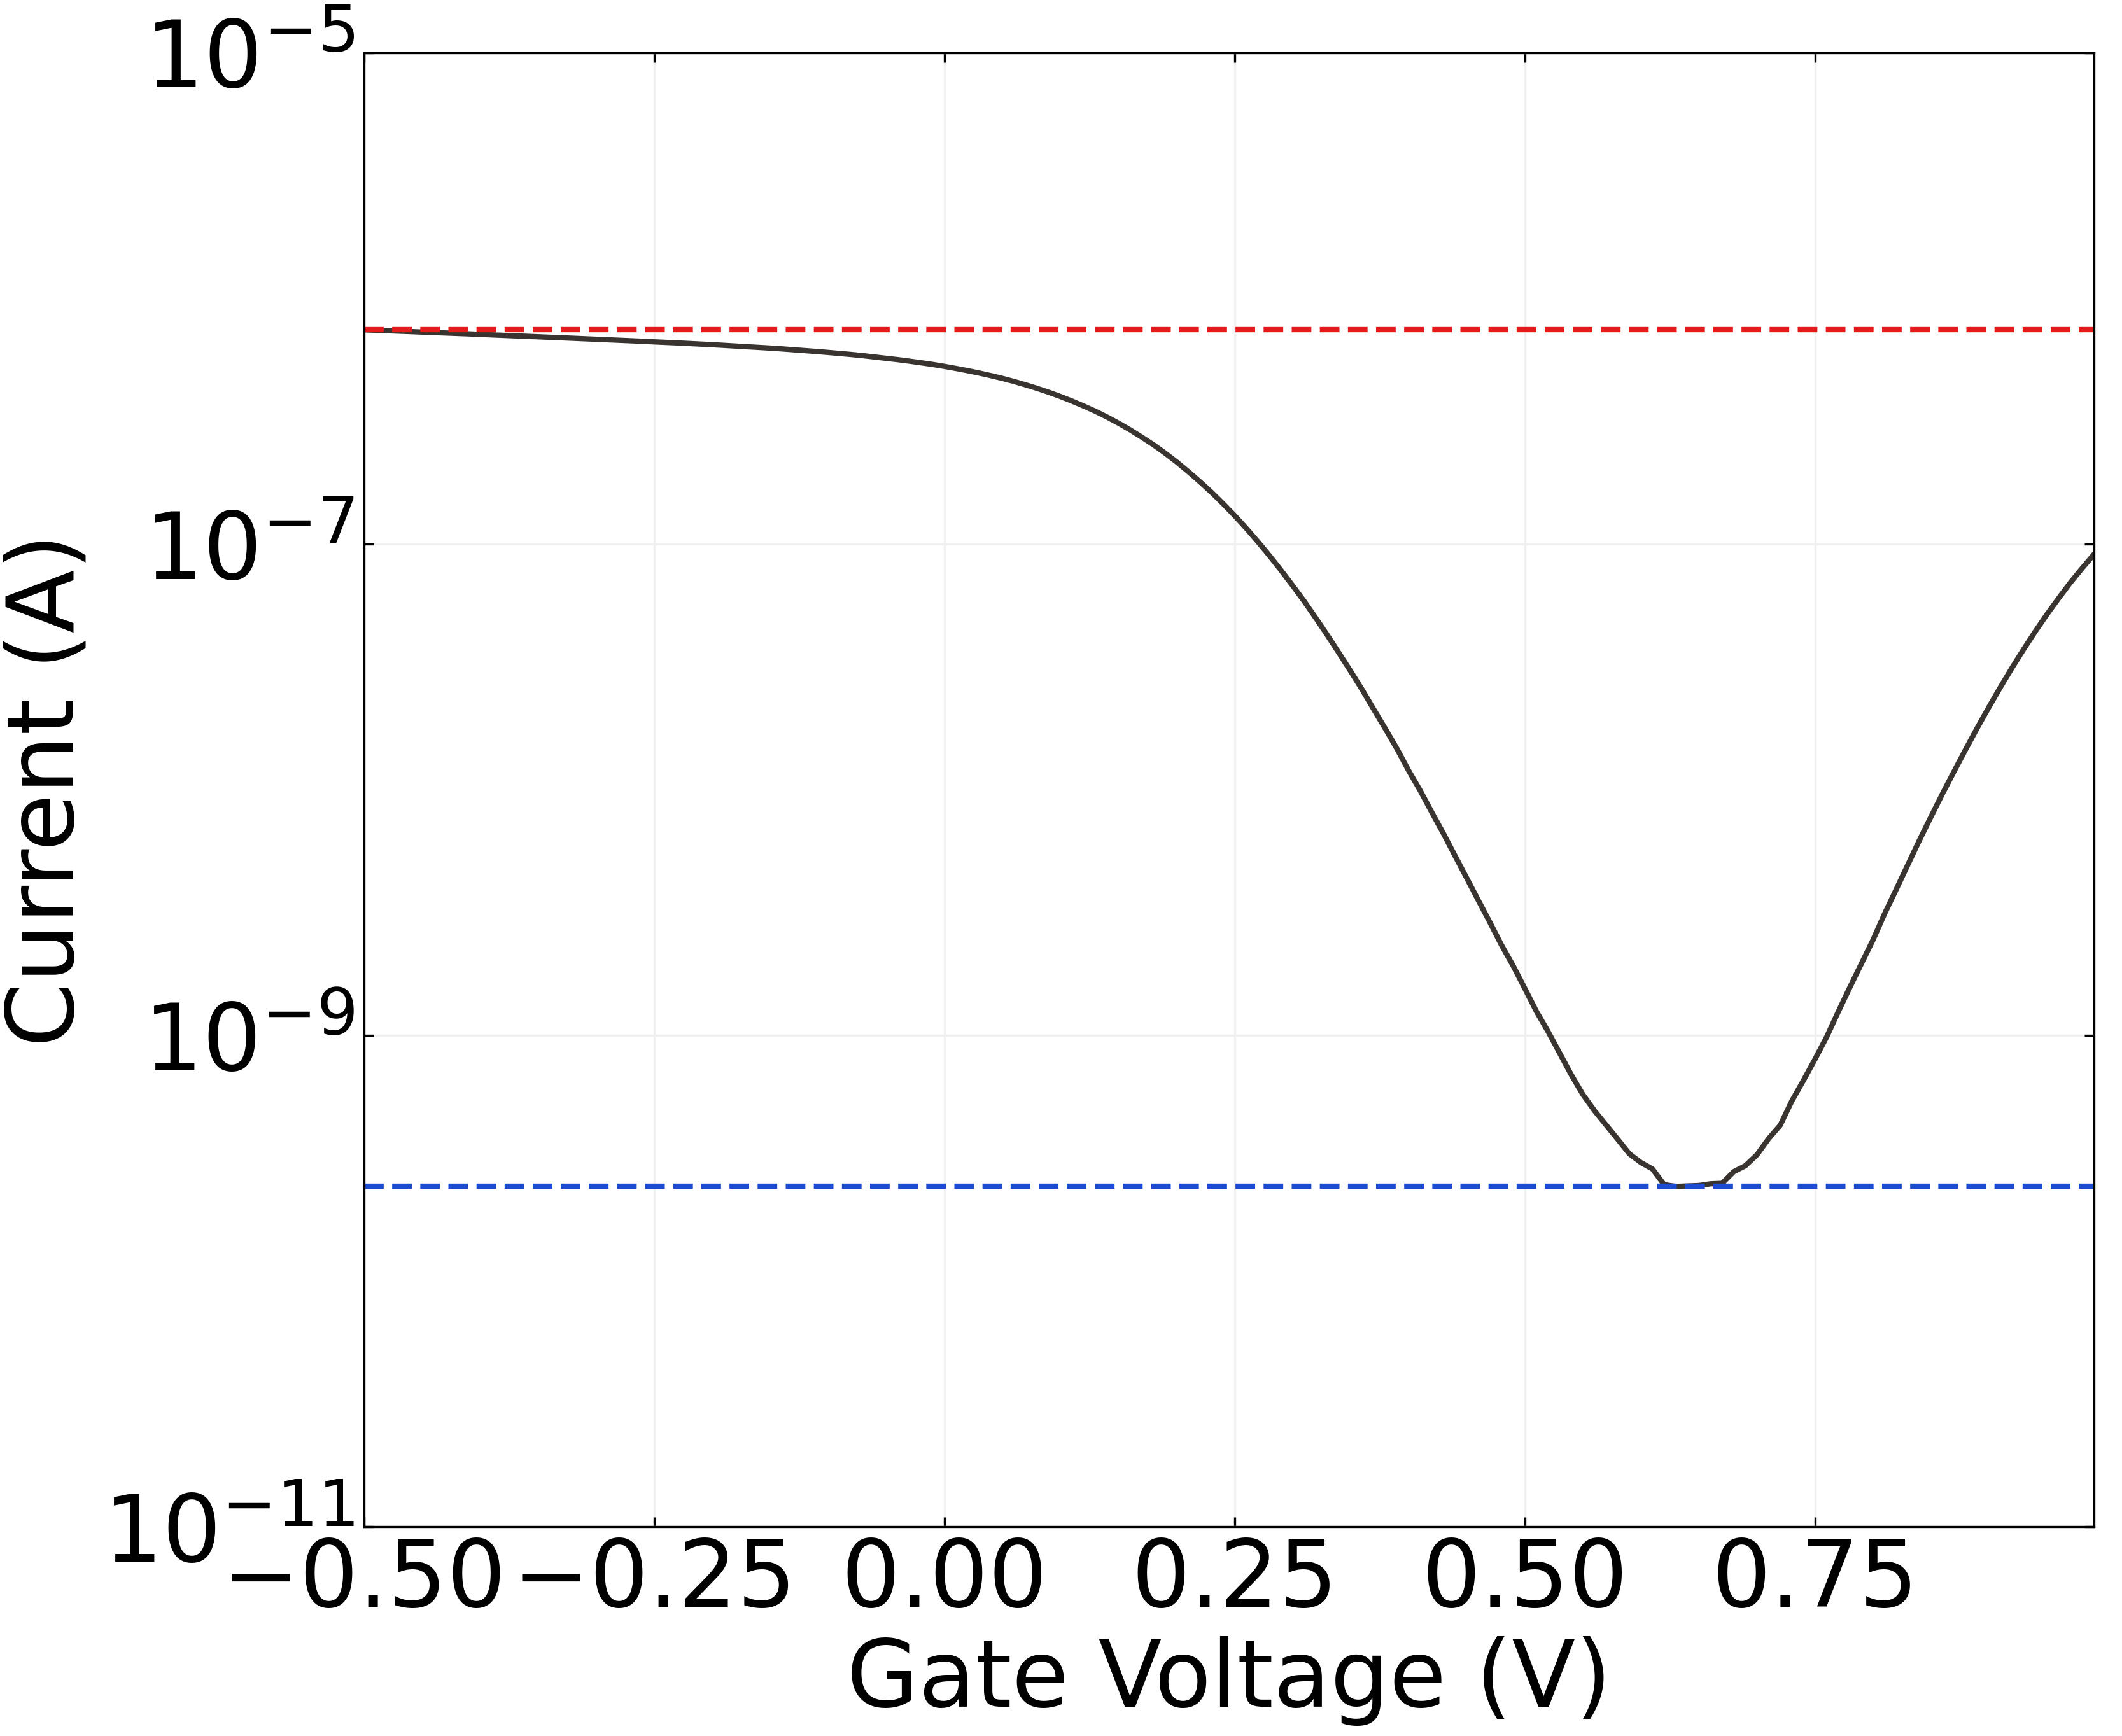
\includegraphics{figures/ch2/NTQ31C5ch1on_off_current.png}\end{minipage}%
%
\begin{minipage}{0.01\linewidth}
~\end{minipage}%

\caption{\label{fig-gating-transfer}Examples of field-effect transistor
transfer characteristics taken at \(V_{ds}\) = 100 mV using two carbon
nanotube network device channels fabricated in the same manner. A linear
scale is used in (a) and (b), while a logarithmic scale is used in (c)
and (d). The curves in (a) and (c) are from a backgated channel, while
the curves in (b) and (d) are from a liquid-gated channel. The linear
fit with gradient corresponding to transconductance at \(V_g\) = 0 V is
shown in (a) and (b) with a dotted red line. The ``on'' current in (c)
and (d) is shown with a red horizontal line, while the ``off'' current
is shown with a blue horizontal line.}

\end{figure}%

The linear and saturation regions for a metal oxide thin-film transistor
are shown in Figure~\ref{fig-linear-region}. In this thesis, constant
\(V_g\) measurements from thin-film transistors were typically taken
when \(V_{ds}\) was small and the TFT was in the linear operation
regime. Figure~\ref{fig-gating-transfer} (a) and (c) show back-gated
transfer characteristics of a thin-film transistor, and
Figure~\ref{fig-gating-transfer} (b) and (d) show liquid-gated TFT
transfer characteristics. The back-gated device exhibits unipolar
behaviour, where the transistor conducts in only one direction along the
\(I_d - V_g\) curve, while the liquid-gated device exhibits ambipolar
behaviour, where conduction occurs along both directions of the curve.
The liquid-gated device is also able to traverse a wide range of
currents over a much more limited voltage interval than the back-gated
device. A variety of quantitative parameters or figures of merit can be
extracted from the transfer characteristics of a thin-film transistor
{[}@Petti2016{]}. Transconductance and on-off ratio are discussed below,
while threshold voltage and subthreshold swing are discussed for the
carbon nanotube network case in
Section~\ref{sec-electrical-characterisation-CNT}.

One of the most important figures of merit which can be extracted from
the transfer characteristic curve of a thin-film FET is the on-off
current ratio, the ratio of the current through a device when the
transistor is gated fully `on', \(I_{on}\), to the current \(I_{off}\)
when gated fully `off'. {[}@Kauffman2008;@Petti2016; @Shkodra2021{]}.
Having a low off current is desirable as it corresponds to low power
consumption by the transistor {[}@Rouhi2010{]}. In
Figure~\ref{fig-gating-transfer} (a), there is a clear on regime at
large negative voltages and an off regime at large positive voltages.
Although the transfer curve never completely flattens in each direction,
\(I_{on}\) can be reasonably be estimated by the highest current
obtained, while \(I_{off}\) can be estimated from the lowest current
reading. In an ambipolar FET, such as that shown in
Figure~\ref{fig-gating-transfer} (b), the off current can be defined as
the minimum current during the transfer sweep, where the majority
carrier transitions from being holes to electrons or \emph{vice versa}
{[}@Petti2016; @Zheng2017{]}. For the backgated channel shown in
Figure~\ref{fig-gating-transfer} (a), the on-off ratio
\(I_{on}/I_{off}\) is \(\sim\) 700, while for the liquid-gated device in
Figure~\ref{fig-gating-transfer} (b), \(I_{on}/I_{off} \sim 3000\). The
superior on-off ratio is a significant advantage of the liquid-gated
configuration {[}@Shkodra2021{]}.

In the linear regime, transconductance at a specific gate voltage is
given by \(g_m = |dI_{d}/dV_g|\). Transconductance indicates how
responsive the device is to electrostatic gating at a given gate
voltage. In other words, when \(g_m\) is large, small changes in \(V_g\)
can significantly modulate channel current \(I_d\), which is useful for
sensing {[}@Heller2009a; @Ohno2015; @Kireev2017{]}. Transconductance at
a given gate voltage is also proportional to the mobility (movement) of
charge carriers in the device channel, and therefore depends on the
scattering properties of the material {[}@Rouhi2010; @Petti2016;
@Li2023{]}. The transconductance at a specific gate voltage can be found
from performing a linear fit in a small region around that voltage on
the transfer curve. Linear fits for transconductance at \(V_g = 0\) V,
the operating voltage used for sensing in this thesis, are shown for a
back-gated device in Figure~\ref{fig-gating-transfer} (a), and a
liquid-gated device in Figure~\ref{fig-gating-transfer} (b). The
corresponding transconductance values of \(g_m\) = 0.002 µS and \(g_m\)
= 1 µS respectively. The difference of several orders of magnitude
between back-gated and liquid-gated transconductance corresponds to the
difference of several orders of magnitude between back and liquid-gated
gate capacitance {[}@Tran2016; @Shkodra2021{]}. The ability to achieve
high transconductance at relatively low voltage is important for the
creation of low power sensors, which is another advantage of the
liquid-gated setup.

Application of higher voltages to the gate in both the liquid-gate and
back-gate cases can result in significant leakage currents through the
gate. These currents mean that the insulating layer at the gate
producing the capacitive effect no longer acts as an insulator,
adversely affecting transistor behaviour and contributing to sensor
drift that may be mistaken for signal responses to analyte
{[}@Noyce2019; @Shkodra2021; @Albarghouthi2022{]}. In the case of
back-gated devices, gate leakage occurs due to conduction through the
oxide dielectric. If the gate voltage produces an electric field
exceeding the dielectric strength of the oxide, dielectric breakdown can
occur, where the oxide layer no longer acts as an insulator. Breakdown
results from voltage-induced oxygen vacancies in the SiO\(_2\) lattice
forming a conductive path through the insulator {[}@Padovani2017{]}.
Breakdown occured at \(\sim\) 50 V for the back-gated channel in
Figure~\ref{fig-gating-transfer}. In the liquid-gated case, the
electrolyte used determines the appropriate voltage range for electrical
characterisation, since excessive voltages will induce redox reactions.
For water-based electrolytes, gate voltages must be kept within the
\(\pm\) 1 V range {[}@Wang2010; @Ohno2015; @Shkodra2021{]}. In normal
operation, gate current should appear negligible on a linear scale, as
shown in Figure~\ref{fig-gating-hysteresis}.

\begin{figure}

\begin{minipage}{0.03\linewidth}
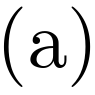
\includegraphics{figures/(a).png}\end{minipage}%
%
\begin{minipage}{0.01\linewidth}
~\end{minipage}%
%
\begin{minipage}{0.45\linewidth}
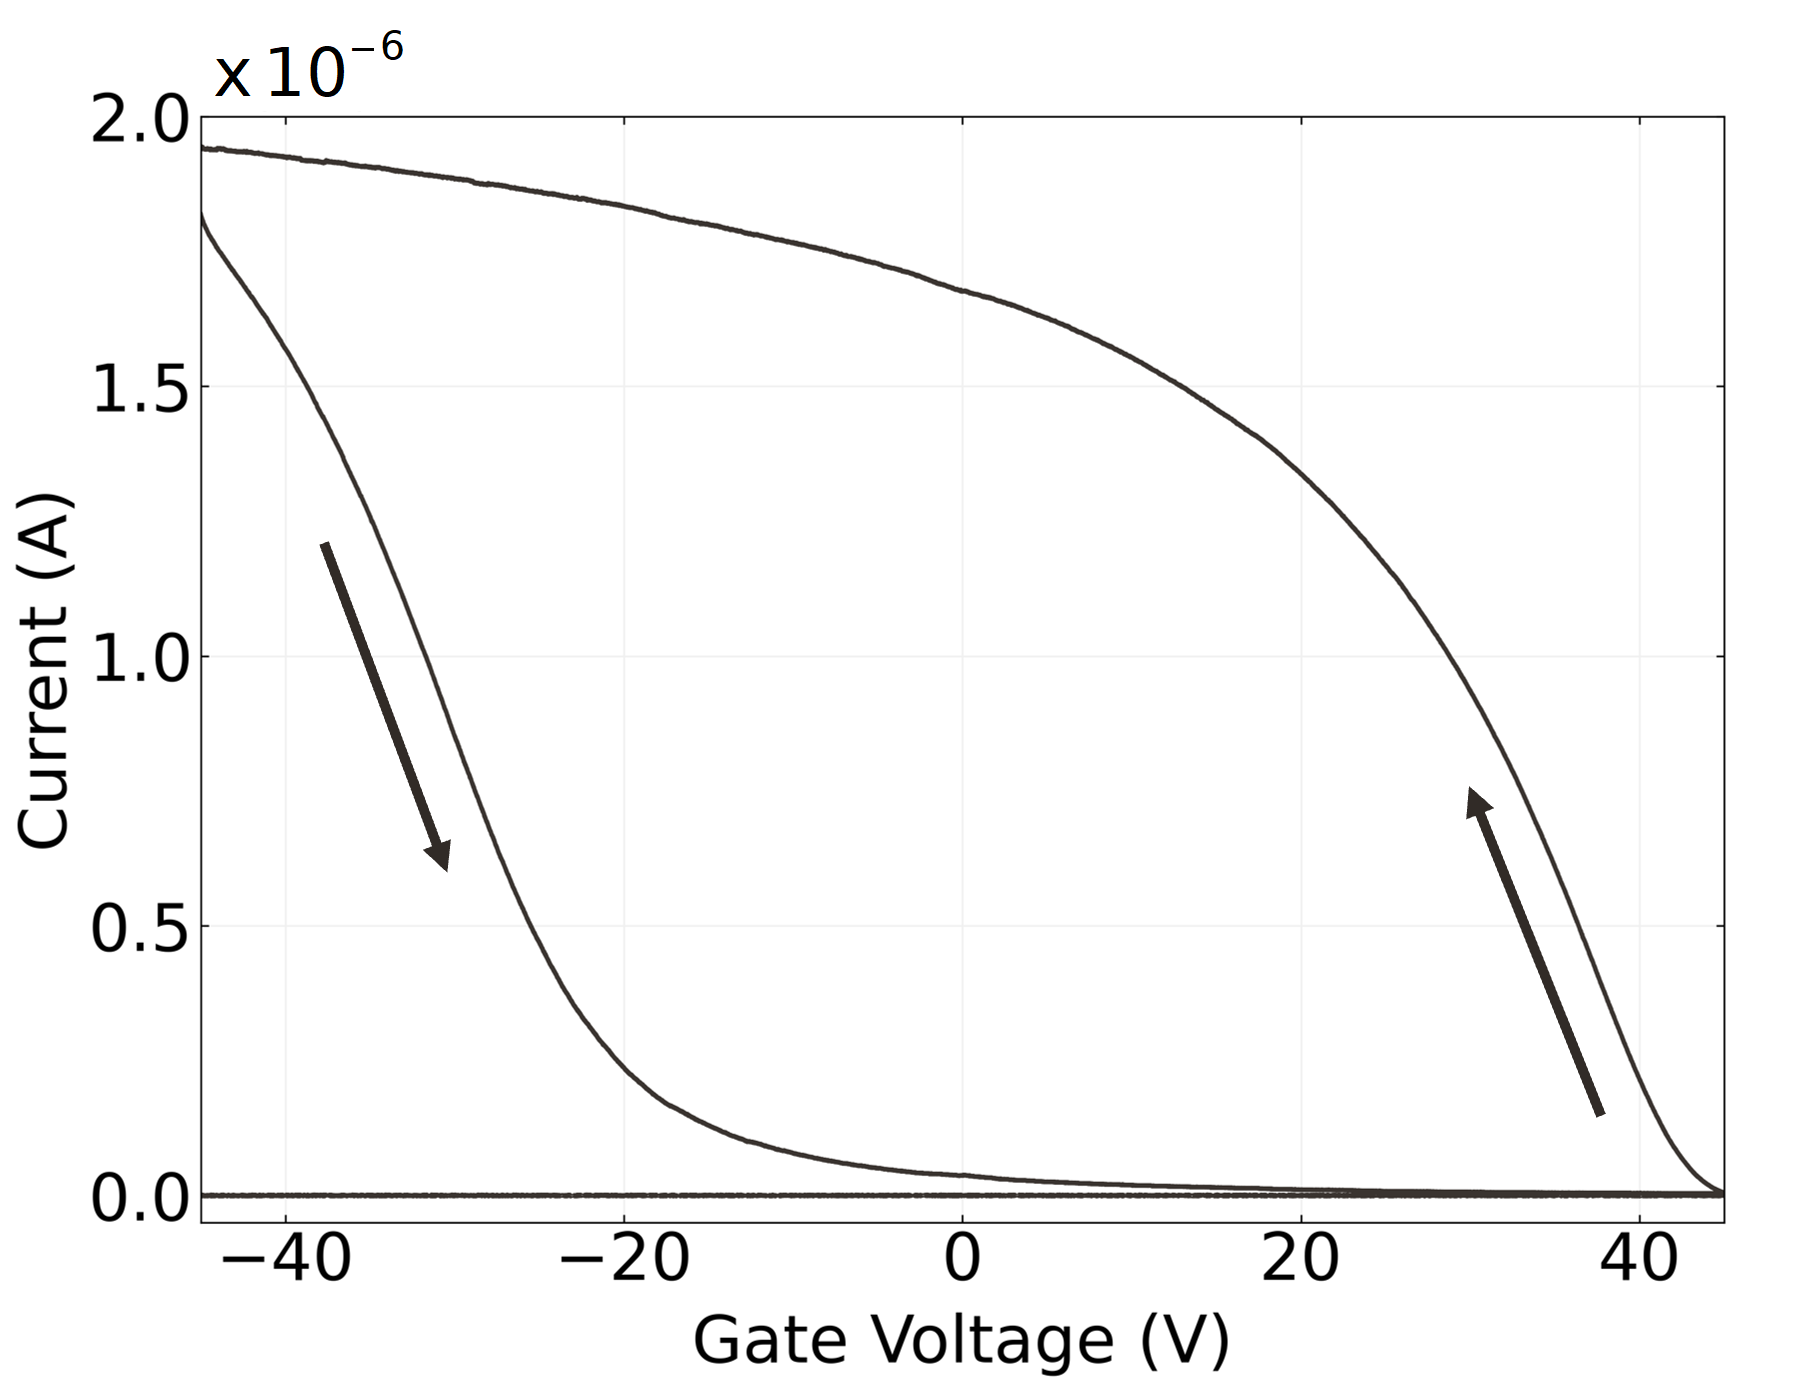
\includegraphics{figures/ch2/Q5C10_hysteresis.png}\end{minipage}%
%
\begin{minipage}{0.01\linewidth}
~\end{minipage}%
%
\begin{minipage}{0.03\linewidth}
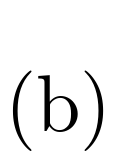
\includegraphics{figures/(b).png}\end{minipage}%
%
\begin{minipage}{0.01\linewidth}
~\end{minipage}%
%
\begin{minipage}{0.45\linewidth}
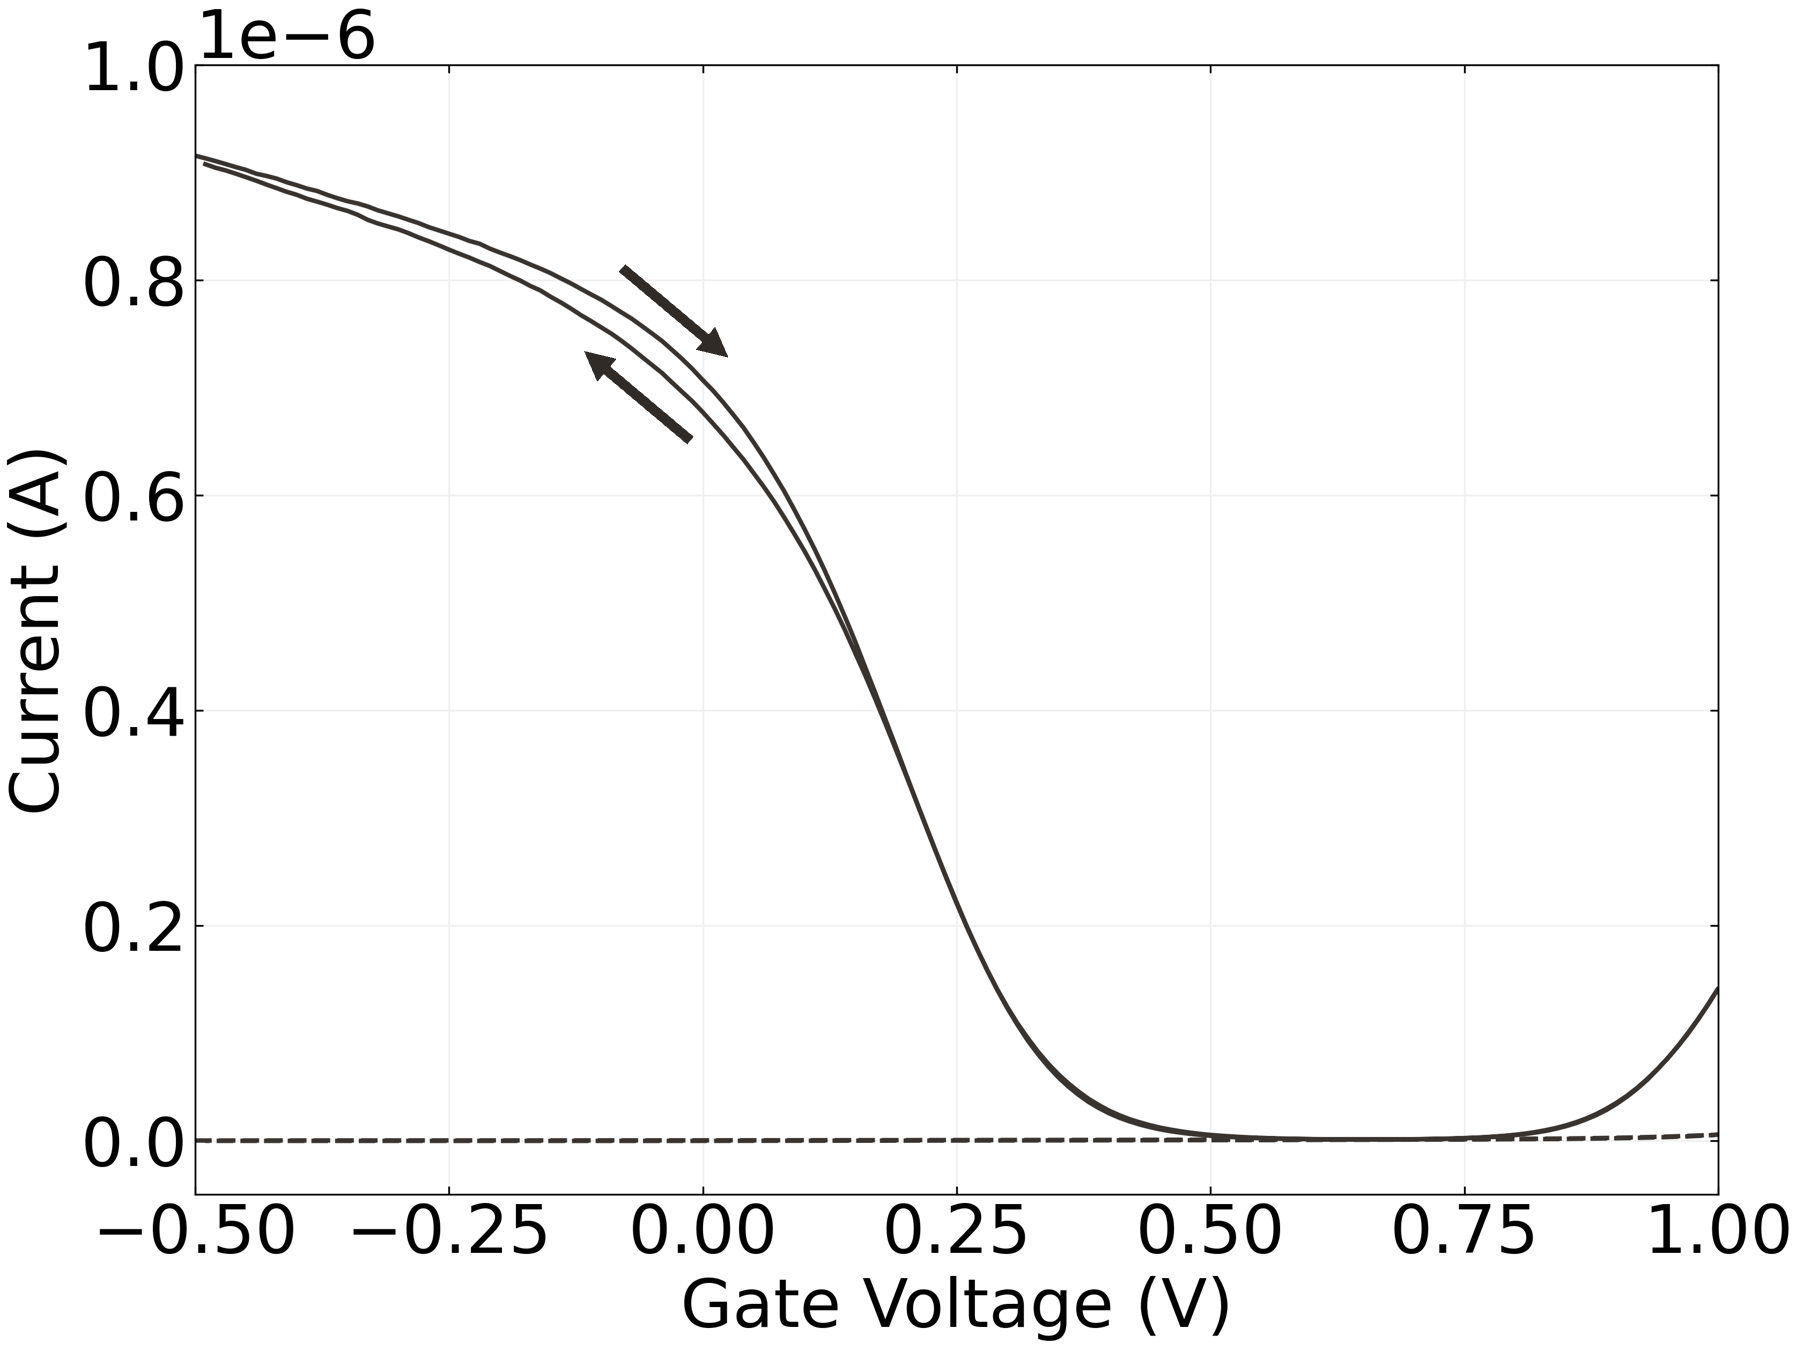
\includegraphics{figures/ch2/NTQ31C5_hysteresis.png}\end{minipage}%
%
\begin{minipage}{0.01\linewidth}
~\end{minipage}%

\caption{\label{fig-gating-hysteresis}Field-effect transistor transfer
characteristics taken at \(V_{ds}\) = 100 mV from two different device
channels on a linear scale. Forward and reverse sweeps are shown for the
back-gated case (a) and the liquid-gated case (b), with the direction of
each sweep indicated by an arrow. A sweep rate of \(V_{ds}\) = 10
mV/sample was used for both transfer curves. The gate current measured
during each sweep is also shown with a dotted line.}

\end{figure}%

Thin-film transistor devices typically exhibit some degree of
hysteresis, where the history of channel current affects future current
behaviour. Hysteresis in carbon nanotube and graphene field-effect
transistors is a result of filling or emptying of slow-discharge charge
traps in the channel environment. These charge traps effectively dope
the SiO\(_2\) insulator or the insulator-channel interface, which
results from gate bias stress or dopant adsorption {[}@McEuen2002;
@Kim2003; @Wang2010; @Bartolomeo2011; @Bargaoui2018; @Peng2018{]}. A
capacitive gating effect from charged ions also contributes to
hysteresis, from the use of a electrolyte-gated environment or from
charged surface contamination {[}@Wang2010; @Yao2021{]}. Due to
hysteresis, sweeping \(V_g\) forwards across a set voltage range will
result in a different \(I_d - V_g\) characteristic curve than
subsequently sweeping over \(V_g\) in the reverse direction. Hysteresis
depends on the voltage range used for characterisation, the sweep rate
and the environment of the transistor channel {[}@Kim2003; @Wang2010{]}.
The effect of hysteresis on \(I_d\) when sweeping gate voltage is shown
in Figure~\ref{fig-gating-hysteresis}. The measured hysteresis is
significantly lower in the liquid-gated case, possibly due to the
smaller voltage range. However, this change may also result from a
reduction in trap states in the SiO\(_2\) layer due to the use of a
liquid-gate.

Memory effects are also present during current measurement when both
source-drain and source-gate voltages are kept constant. These changes
appear as a slow change in current, and are referred to here as either
signal drift or baseline drift. In more extreme cases, baseline drift
can obscure or even be confused with current changes attributable to
analyte interaction during real-time sensing {[}@Noyce2019{]}. Signal
drift occurs both in ambient conditions and in a vacuum environment, and
cannot be accounted for by changes in room temperature and ambient
lighting alone. While research into signal drift is ongoing, it appears
to be a hysteretic effect resulting from changes in trap states over
time {[}@Lin2006; @Bargaoui2018; @Noyce2019{]}. The high demand for
characterisation equipment in a standard device laboratory means that
waiting over three hours for baseline drift to settle is impractical,
and furthermore, extended periods of voltage application may degrade
bio-functionalised devices {[}@Noyce2019{]}. Since trap states are
unavoidable to some extent {[}@DiMaria1993; @Collins2000{]}, data
analysis that accounts for baseline drift was therefore explored in some
detail in this thesis.

\subsection{Graphene Field-Effect
Transistors}\label{graphene-field-effect-transistors}

\subsubsection{Graphene Properties}\label{graphene-properties}

Graphene is a 2-dimensional material which consists of covalently bonded
carbon atoms in a dense lattice of hexagonal cells {[}@McEuen2002;
@Novoselov2004; @Geim2007; @Tran2016{]}. Graphene can be used to create
a variety of low-dimensional graphitic nanomaterials, including carbon
nanotubes {[}@McEuen2002{]} (see Section~\ref{sec-carbon-nanotubes}).
Monolayer and bilayer graphene are zero band-gap semiconductors, where
traversing the electronic bandstructure in different directions gives
rise to either metallic or semiconducting behaviour {[}@McEuen2002;
@Peng2018{]}. Adding more graphene layers adds more complexity to the
bandstructure, with significant overlap between bands and reduced
carrier mobility. When 10 or more layers are present, the structure
behaves as 3-dimensional graphite {[}@Geim2007; @Ohno2015{]}. First
isolated and used as a thin-film transistor channel in 2004
{[}@Novoselov2004{]}, monolayer graphene has many desirable electronic
properties. Charge carrier transport is ballistic over submicrometer
distances at room temperature, and as graphene is metallic even at the
Dirac point, this transport is not inhibited by a Schottky barrier at
the metal contacts of a device {[}@Novoselov2004; @Geim2007;
@Peng2018{]}. Graphene is also a highly chemically stable material. In
particular, it will not readily oxidise in an electrolyte solution due
to having a large `electrochemical window'; in other words, it is too
chemically stable to take part in electrochemical reactions within a
large range of applied voltages {[}@Ohno2015; @Tran2016{]}.

\paragraph*{Graphene Folds}\label{graphene-folds}
\addcontentsline{toc}{paragraph}{Graphene Folds}

\begin{figure}

\centering{

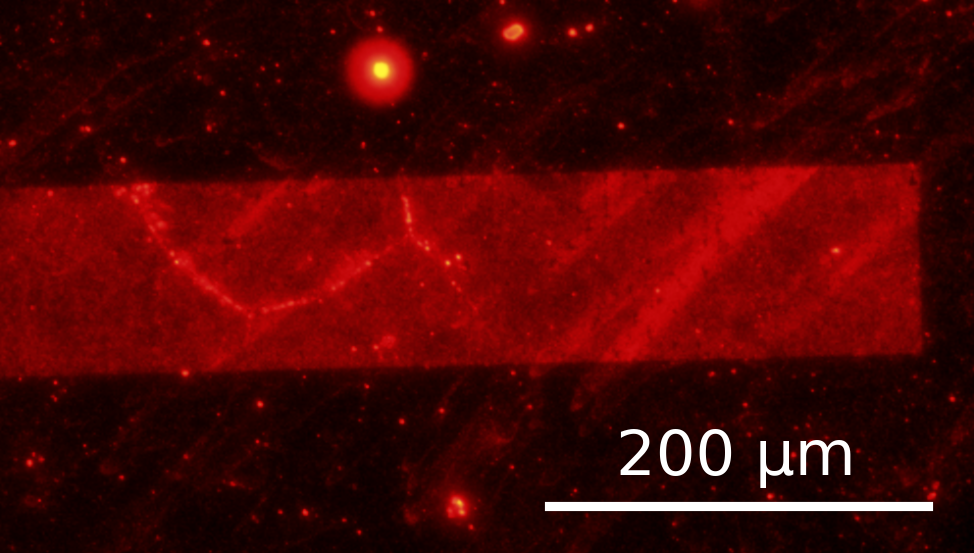
\includegraphics[width=0.5\textwidth,height=\textheight]{figures/ch2/modified_NGW8D4_1mM_rhodamineB_centralchannel3_postMsurfactantclean5min_2.4sexposure_20X_221111.png}

}

\caption{\label{fig-graphene-folds}Fluorescence image of a strip of
graphene on SiO\(_2\) surface functionalised with Rhodamine B dye.
Bright lines are visible on the left side of the graphene surface which
correspond to preferential attachment of dye along the graphene folds.}

\end{figure}%

Graphene folding (also referred to as warping or wrinkling) of up to
\(\sim\) 6 nanometers in height occurs at many locations on a graphene
monolayer {[}@Zhu2012{]}. These folds primarily result from the chemical
vapour deposition (CVD) process onto copper used in the creation of
graphene films. The thermal contraction of copper exceeds that of
graphene during the rapid cooling that takes place after deposition.
Since the graphene is pinned to the surface, this leads to slight
folding of the monolayer {[}@Zhao2012; @Zhu2012; @Chhikara2013{]}.
Transferring graphene from the rough copper to a relatively smooth
Si/SiO\(_2\) wafer may also contribute to wrinkling {[}@Zhao2012;
@Kireev2017{]}. These folds help to mechanically stabilise the graphene
layer, but have significant negative effects on charge transport
{[}@Geim2007; @Chhikara2013; @Zhu2012{]}. Folds also exhibit enhanced
reactivity due to their low radius of curvature {[}@Zhao2012{]}. This is
demonstrated in Figure~\ref{fig-graphene-folds}, where the fluorescent
Rhodamine B dye preferentially bonds to folded regions, leading to
particularly dense functionalisation in these regions. This behaviour
has previously been observed for the decoration of graphene with
pentacene molecules {[}@Chhikara2013{]}. Other defects influencing
surface reactivity include grain boundaries and point defects in the
crystal structure {[}@Zhao2012; @Chhikara2013; @Kireev2017{]}.

\subsubsection{Electrical
Characterisation}\label{sec-electrical-characterisation-graphene}

The transfer sweep behaviour of a graphene device is ambipolar and has
no off regime under standard conditions {[}@Novoselov2004;
@Bartolomeo2011; @Ohno2015{]}. When a gate voltage \(V_g\) is applied to
the channel of a graphene device, the Fermi energy of the graphene is
shifted and surface charge density is altered {[}@Novoselov2004;
@Heller2010; @Ohno2015{]}. An increase in surface charge density means
an increase in carriers available for either \(p\) or \(n\)-conduction
and increased \(I_d\) {[}@Geim2007{]}. The regions of hole conduction
and electron conduction are shown in
Figure~\ref{fig-graphene-characteristics} (a), alongside the
corresponding Fermi energy on the simplified graphene bandstructure
(known as a `Dirac cone'). The transconductance of the curve at \(V_g\)
= 0 V, \(g_m\) = 1 µS, is similar to the liquid-gated transconductance
of a carbon nanotube device shown earlier. As graphene lacks a bandgap,
there is a minimum possible conductance for graphene devices, which
leads to a relatively small on-off ratio {[}@Novoselov2004;
@Geim2007{]}. Folding may further decrease on-off ratio due to diffusive
transport of carriers along the folds {[}@Zhu2012{]}. The on-off ratio
of the graphene transfer curve shown in
Figure~\ref{fig-graphene-characteristics} (a) is 5. A bandgap can be
introduced to a graphene device using a dual-gated configuration,
increasing the on-off ratio past 100 {[}@Xia2010{]}.

\begin{figure}

\begin{minipage}{0.03\linewidth}
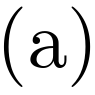
\includegraphics{figures/(a).png}\end{minipage}%
%
\begin{minipage}{0.01\linewidth}
~\end{minipage}%
%
\begin{minipage}{0.45\linewidth}
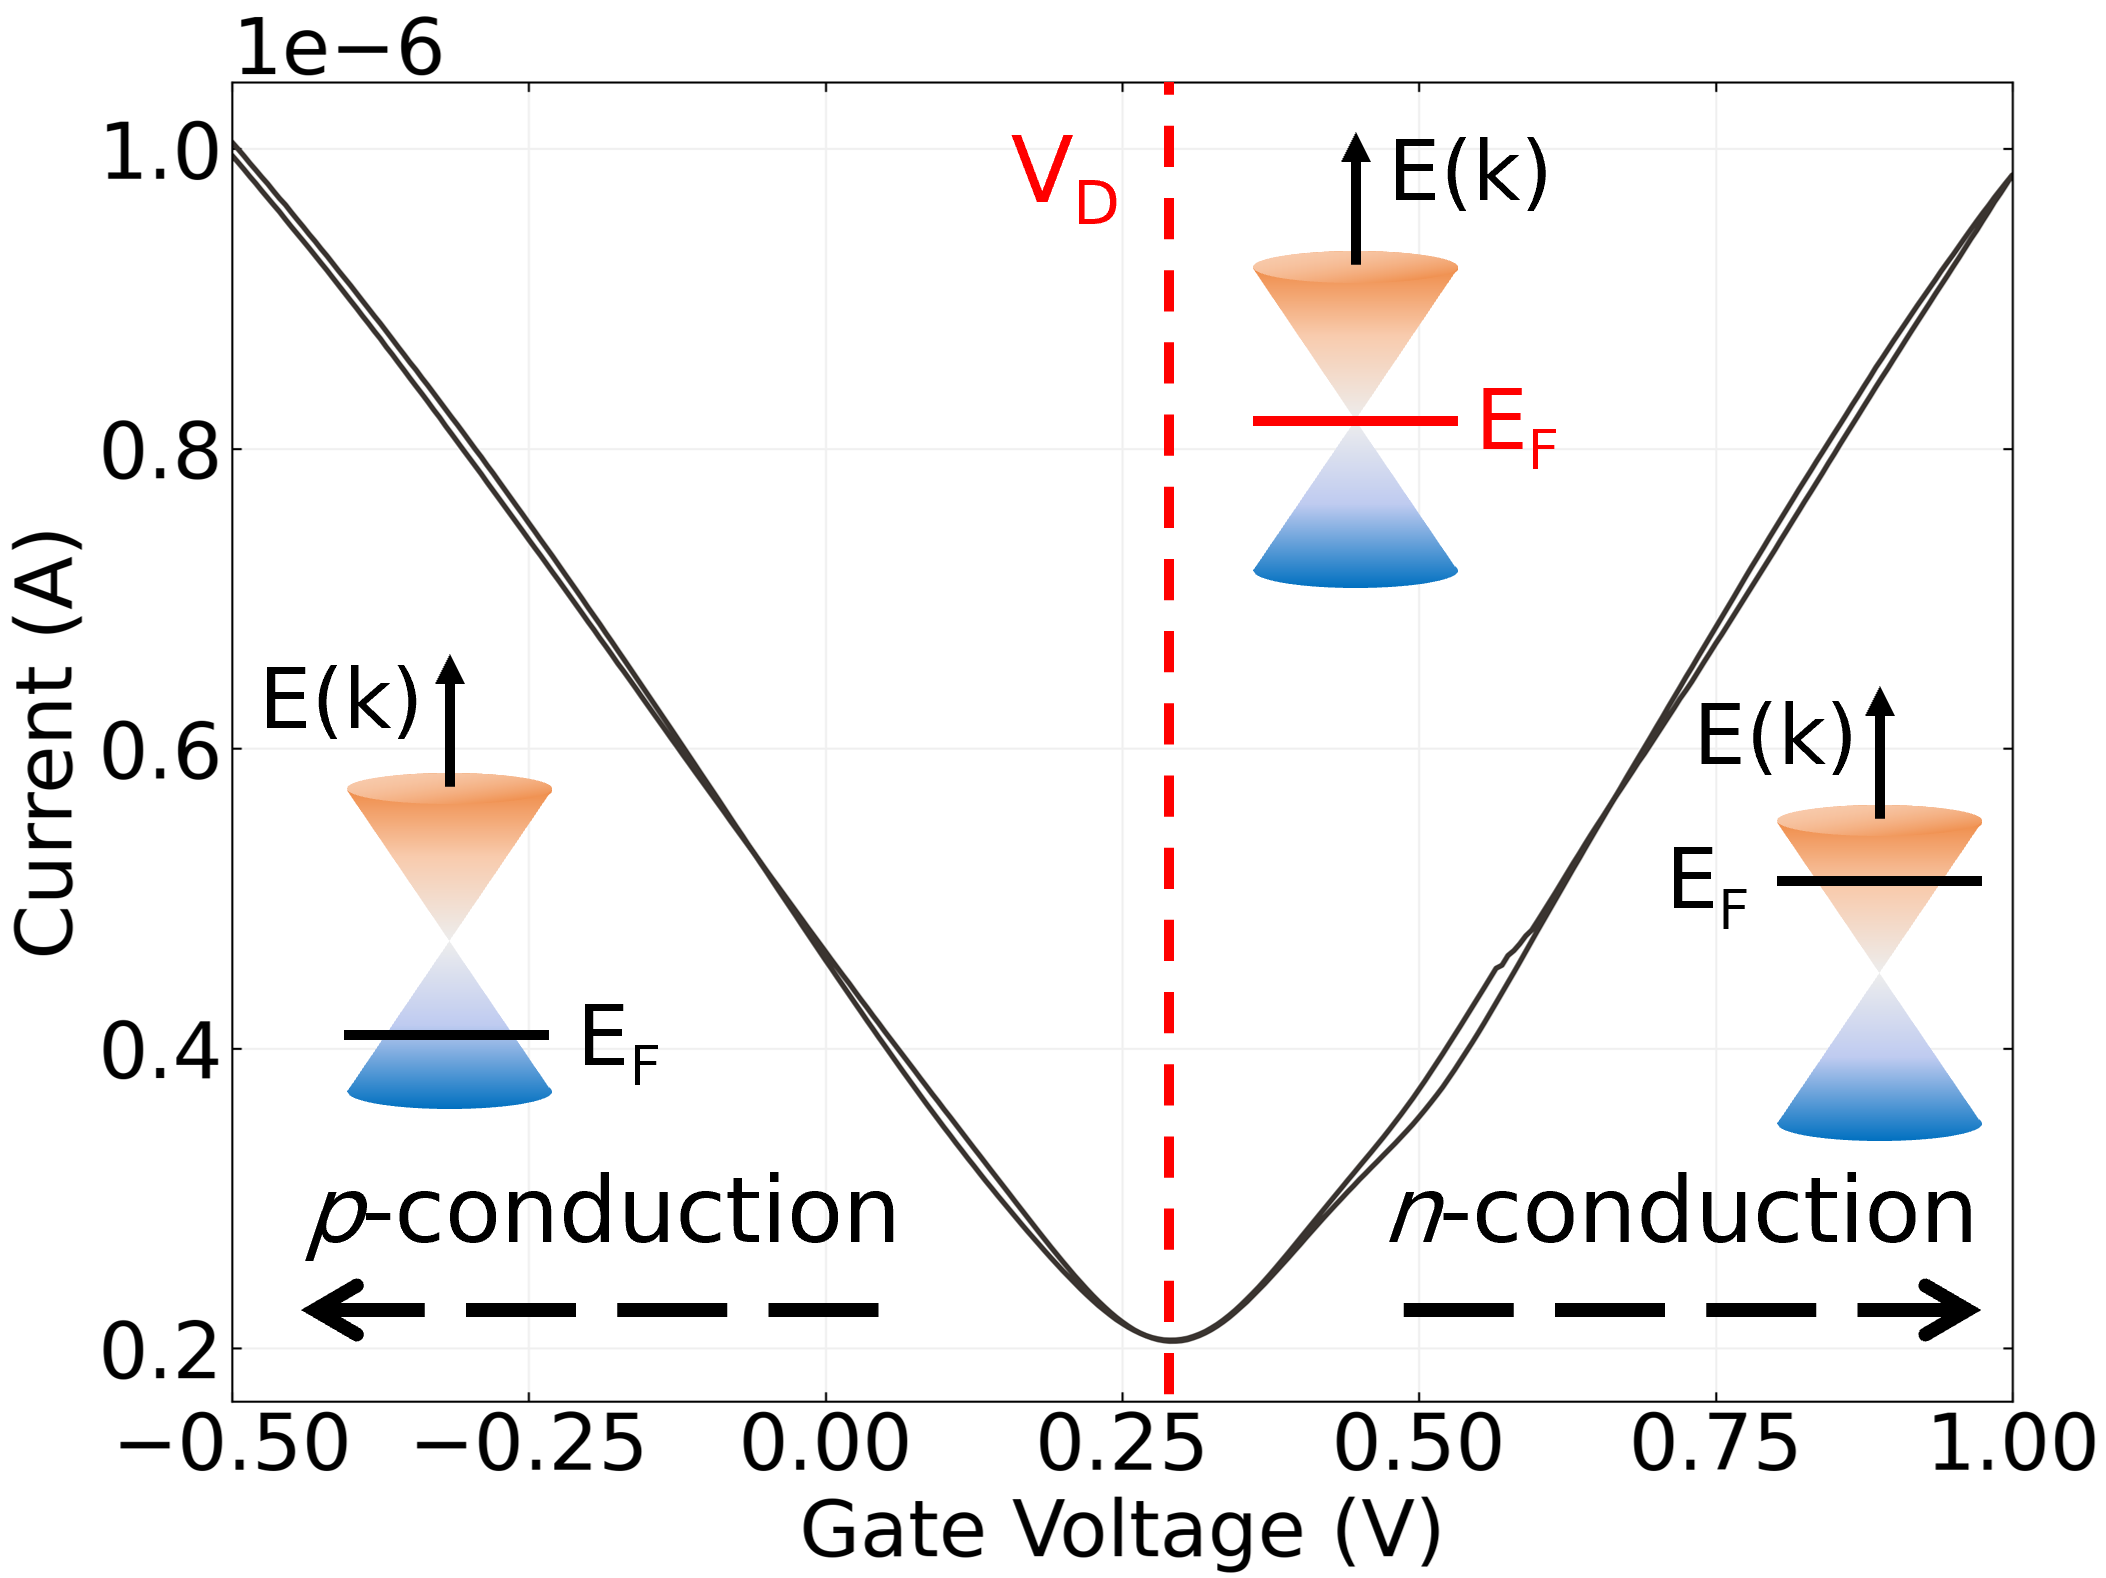
\includegraphics{figures/ch2/Graphene_transfer_1.png}\end{minipage}%
%
\begin{minipage}{0.01\linewidth}
~\end{minipage}%
%
\begin{minipage}{0.03\linewidth}
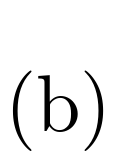
\includegraphics{figures/(b).png}\end{minipage}%
%
\begin{minipage}{0.01\linewidth}
~\end{minipage}%
%
\begin{minipage}{0.45\linewidth}
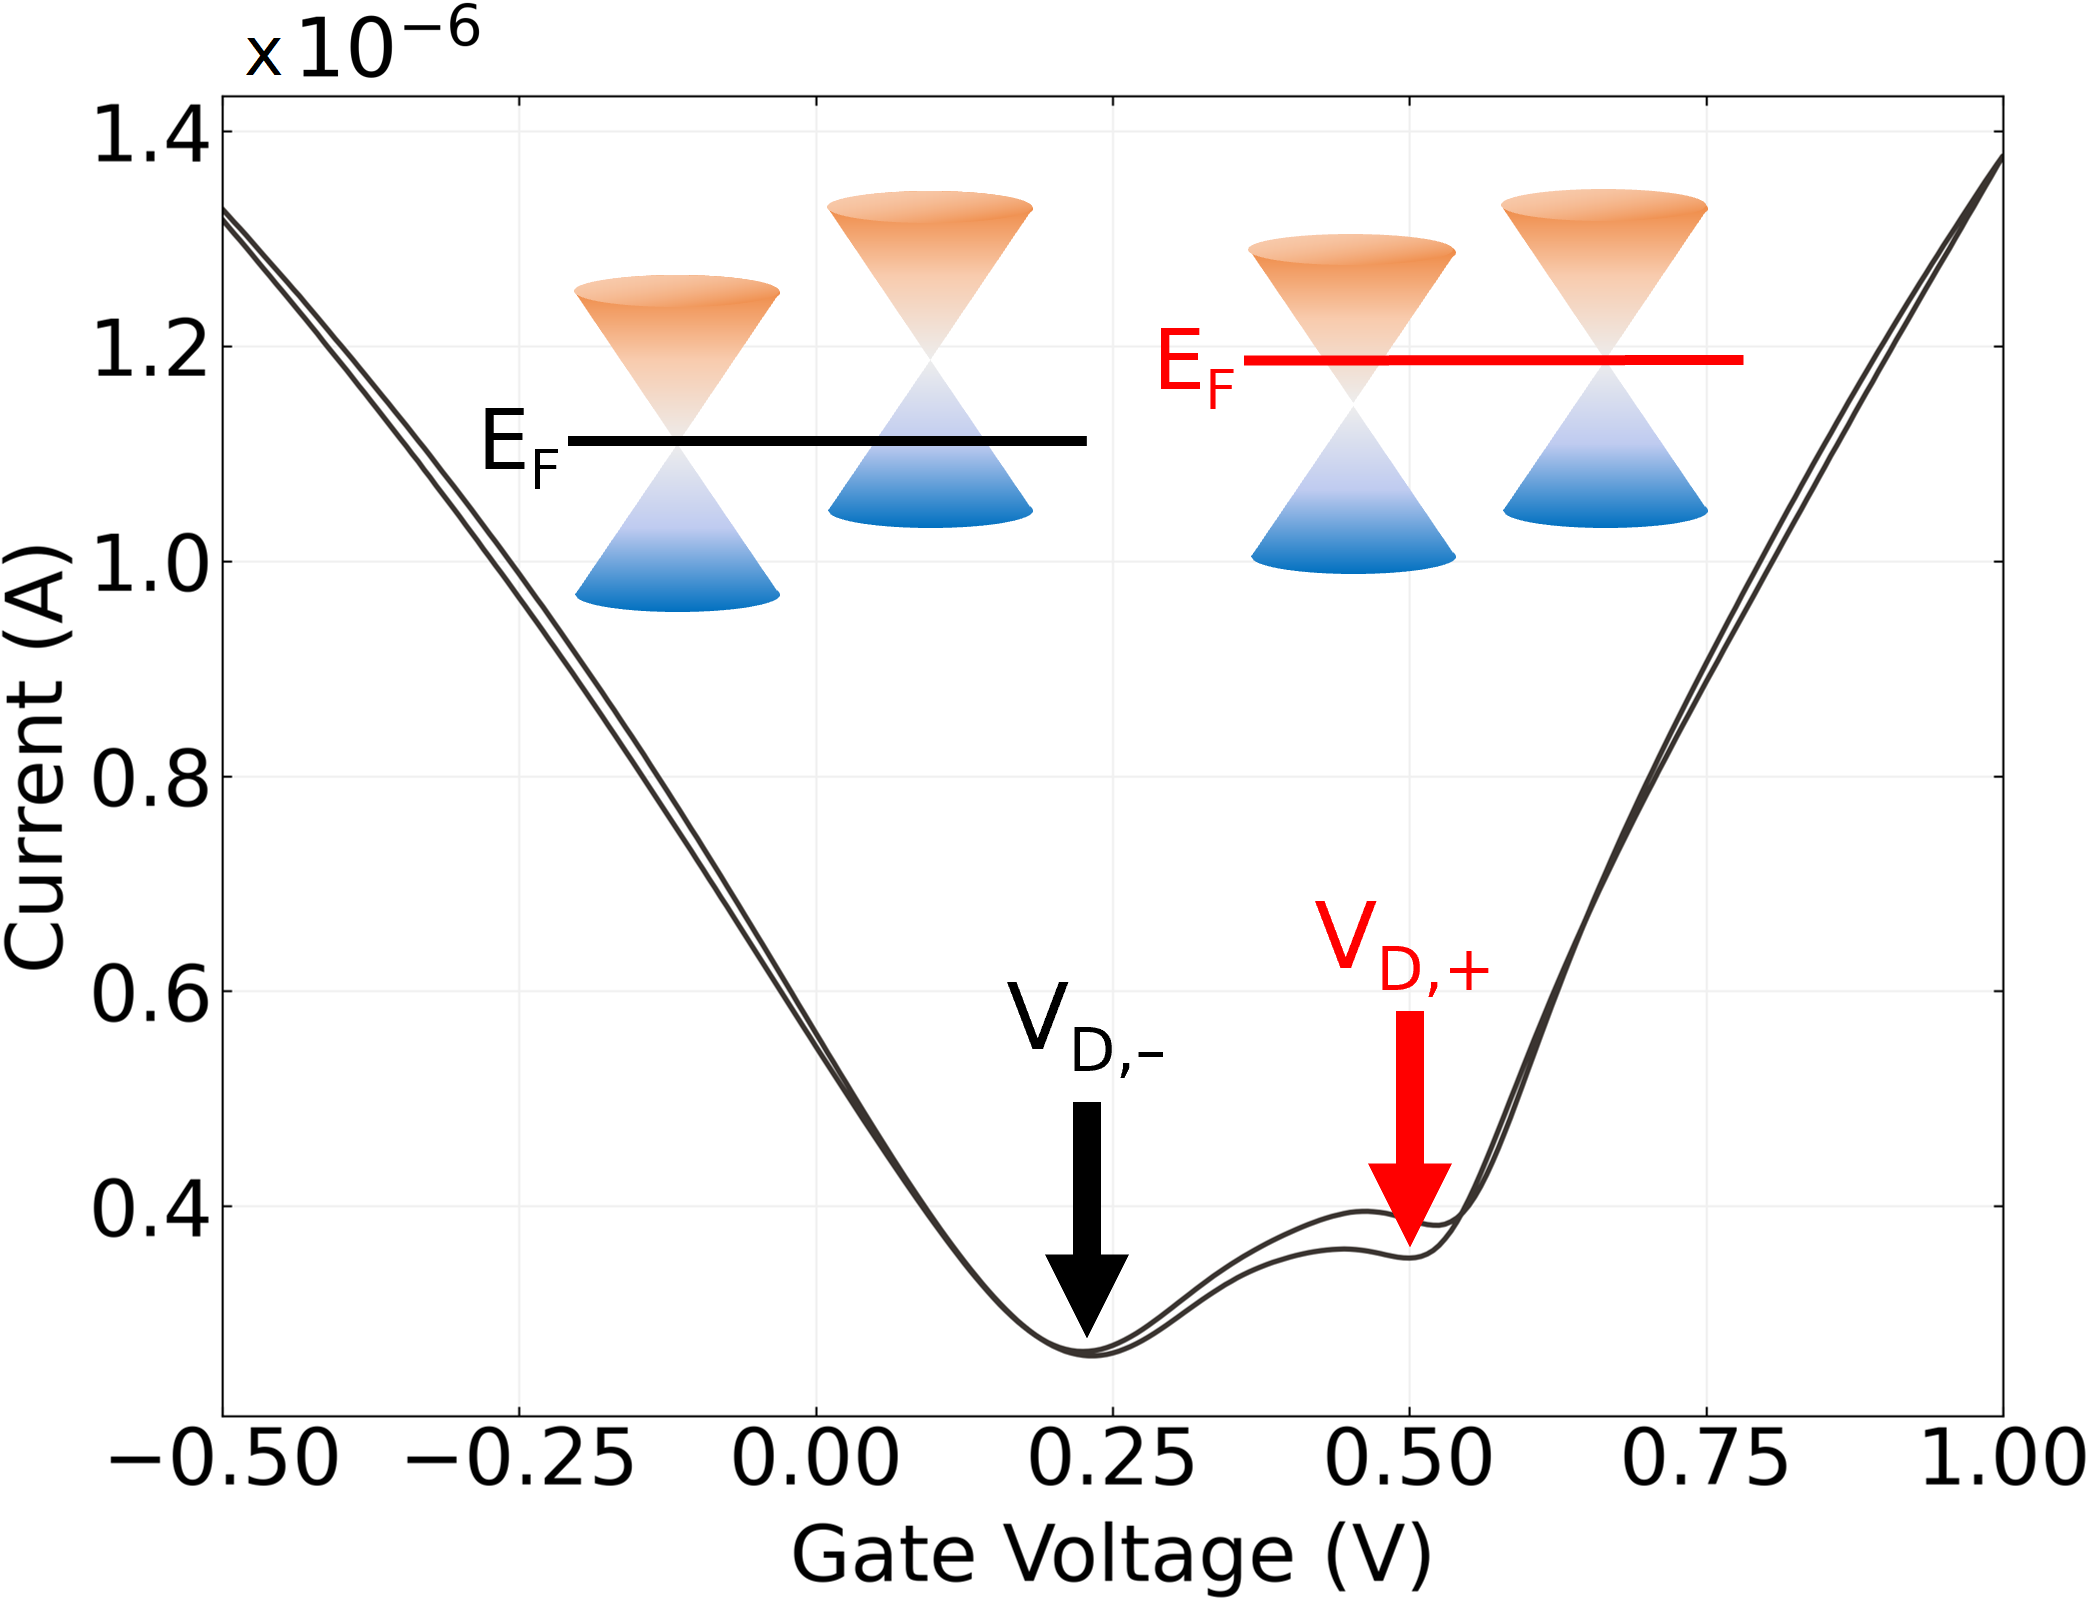
\includegraphics{figures/ch2/Graphene_transfer_2.png}\end{minipage}%
%
\begin{minipage}{0.01\linewidth}
~\end{minipage}%

\caption{\label{fig-graphene-characteristics}Liquid-gated transfer
characteristics of two graphene field-effect transistor channels. In
(a), the Dirac point voltage is indicated by a red dotted line, and
regions of hole conduction and electron conduction are also shown. The
relative Fermi energy in each region is shown on graphene bandstructure
insets (Adapted from {[}@Geim2007; @Ohno2015{]}). The graphene channel
in (b) has double conduction minima, which are highlighted with red
arrows. The relative Fermi energy at each minima is also shown on
bandstructure insets (Adapted from {[}@Peng2018{]}).}

\end{figure}%

The minimum conductance obtainable by gating in a graphene device occurs
at what is known as the charge neutrality or Dirac point, where the
population of charge carriers is at a minimum {[}@Novoselov2004;
@Bartolomeo2011; @Ohno2015; @Kireev2017{]}. At gate voltages close to
the Dirac voltage, both electrons and holes are present, and at the
Dirac point, there are equal concentrations of each carrier present
{[}@Novoselov2004; @Bartolomeo2011; @Peng2018{]}. As shown in
Figure~\ref{fig-graphene-characteristics} (a), as the gate voltage moves
left away from the Dirac voltage and Fermi energy is shifted into the
valence band, holes begin to dominate conduction, while as gate voltage
is moved to the right of the Dirac voltage, where Fermi energy is
shifted into the conduction band, electrons dominate {[}@Novoselov2004;
@Bartolomeo2011; @Feng2014; @Zhang2015{]}. At points far from the Dirac
voltage, conductivity increases linearly {[}@Novoselov2004;
@Bartolomeo2011; @Peng2018{]}. Typically, a monolayer graphene channel
conducts holes at zero gate voltage, which results from the presence of
\(p\)-dopants such as oxygen and water adsorbed from the air and resist
residues. By removing these dopants, the Dirac point feature can be
brought closer to the zero gate voltage position on the transfer curve,
indicating graphene is naturally a mixed-carrier conductor
{[}@Novoselov2004; @Bartolomeo2011; @Zhang2015; @Kireev2017;
@Peng2018{]}.

Some graphene devices naturally exhibit a double-minimum feature in the
transfer characteristic curve, corresponding to two separate Dirac
points {[}@Bartolomeo2011; @Feng2014; @Zhang2015; @Kireev2017;
@Peng2018{]}. This effect is due to doping of graphene by charge
transfer from the metal contacts. In shorter length channels, metal
doping affects the entire channel length. Band bending from channel
doping near the metal contact results in a consistent Fermi level across
the channel, meaning only a single Dirac point is present in the
transfer characteristic curve. However, for longer channels, metal
doping no longer occurs across the entire channel length
{[}@Bartolomeo2011; @Peng2018{]}. This discrepancy leads to a difference
in Fermi level between the metal-doped graphene and graphene in the
unaffected channel region {[}@Bartolomeo2011; @Feng2014; @Peng2018;
@Zhang2015{]}. The difference in Fermi levels results in the
introduction of a second Dirac point. The relative level of doping in
the metal-doped and unaffected channel regions determines the relative
\(V_g\) position of each local minimum on the \(I_d - V_g\) curve
{[}@Bartolomeo2011; @Peng2018; @Zhang2015{]}.

Figure~\ref{fig-graphene-characteristics} (b) shows a double-minimum
transfer characteristic with each Dirac point indicated. At large
negative \(V_g\), the Fermi energy level is far from the Dirac point
energy of both the channel and contact regions, and holes dominate
conduction. As \(V_g\) and the Fermi energy approach and then pass the
Dirac point corresponding to the left minimum \(V_{D,-}\), the available
carriers likewise decrease to a minimum and begin to increase again in
one region \(R_1\), but continuously decrease in the other region
\(R_2\). The shape of the curve between \(V_{D,-}\) and the right local
minimum \(V_{D,+}\) then depends on the relative rate of increasing
electron and decreasing hole populations, where the graphene is
\(n\)-doped in \(R_1\) and \(p\)-doped in \(R_2\). At the local minimum
on the right, \(V_{D,+}\), the carriers in \(R_2\) now reach a minimum,
while carriers in \(R_1\) continue to increase. At voltages well beyond
\(V_{D,+}\), electrons then dominate conduction in both regions
{[}@Bartolomeo2011; @Zhang2015; @Peng2018{]}.

\subsubsection{Sensing Behaviour}\label{sensing-behaviour}

The large surface-to-volume ratio of graphene makes it highly sensitive
to intermolecular interactions and therefore appropriate for use in
sensing applications {[}@Ohno2015; @Tran2016{]}. An analyte molecule can
be detected using a graphene channel by observing the change in current
that occurs when the presence of a charged analyte alters the channel
Fermi level {[}@Heller2010; @Ohno2015{]}. Sensing may be dominated by
interactions occurring at the graphene folds {[}@Zhao2012{]}. The small
on-off ratio of graphene is a drawback when used in field-effect
transistor sensing applications when compared with carbon nanotube
transistors {[}@Novoselov2004{]}. If a dual-gate configuration is used,
however, on-off ratio can be increased significantly by introducing a
bandgap. The presence of a bandgap means a Schottky barrier is
introduced at the graphene-electrode interface, whose modulation can
then also contribute as a potential sensing mechanism (see
Section~\ref{sec-cnt-network-details} for a discussion of Schottky
barriers) {[}@Xia2010{]}.

\subsection{Carbon Nanotube Field-Effect
Transistors}\label{carbon-nanotube-field-effect-transistors}

\subsubsection{Carbon Nanotube Properties}\label{sec-carbon-nanotubes}

Since their initial identification in 1991 {[}@Iijima1991{]}, a wide
range of applications for carbon nanotubes (CNTs) have been proposed,
due to their small mass, elasticity, strength, and unique electronic
properties. A single-walled carbon nanotube (SWCNT) consists of a
monolayer graphene sheet rolled up into a cylinder, while a multi-walled
carbon nanotube (MWCNT) consists of several monolayer graphene cylinders
where smaller cylinders are coaxially contained by larger cylinders
{[}@Dekker1999; @Avouris2007; @Cao2009; @Rouhi2010; @Shkodra2021{]}.
Multi-walled carbon nanotubes can suffer from significant scattering at
defects leading to diffusive electron motion {[}@Dekker1999{]}. However,
single-walled carbon nanotubes are relatively defect-free, and carrier
transport within nanotubes is near-ballistic at room temperature,
resulting in high carrier mobility {[}@Dekker1999;@Avouris2007;
@Cao2009; @Rouhi2010; @Shkodra2021{]}. The momentum of charge carriers
in a single-walled carbon nanotube is quantised, confining carriers to
2-dimensional slices across the 3-dimensional graphene bandstructure. If
a slice contains a bandgap, the carbon nanotube behaves as a
semiconductor (s-CNT); if not, the nanotube behaves as a metal (m-CNT)
{[}@McEuen2002{]}. The high surface-to-volume ratio of small-diameter
single-walled carbon nanotubes makes them extremely sensitive and
therefore particularly suitable for sensing applications {[}@Cao2009;
@Yao2021; @Shkodra2021{]}. Like graphene, carbon nanotubes have a large
potential window, and can be used safely in a liquid-gate environment
without undergoing redox reactions {[}@Ohno2015{]}.

\begin{figure}

\centering{

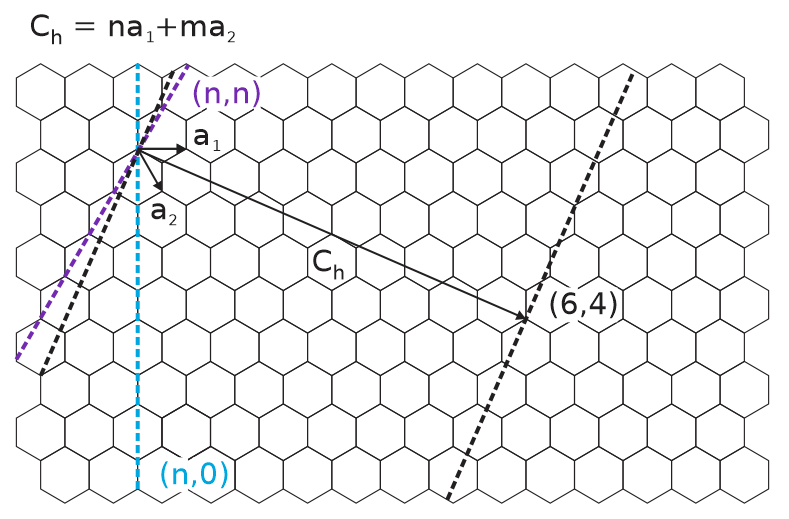
\includegraphics[width=0.55\textwidth,height=\textheight]{figures/ch2/carbon_nanotube_wrapping.png}

}

\caption{\label{fig-carbon-nanotube-wrapping}Diagram illustrating how a
graphene sheet can be rolled up at various angles to form carbon
nanotubes. The two black dotted lines represent boundaries which can be
cut across and then brought into contact to form a cylinder. The
cylinder here is referred to by the integer pair (6,4), as the chiral
vector \(C_h\), the vector perpendicular to the cut through the sheet,
is given by \(C_h = 6a_1+4a_2\). The chiral vector forms the
circumference of the rolled carbon nanotube. The left edge in the zigzag
(\(n\),0) and armchair (\(n\),\(n\)) cases are shown with a blue and
purple dotted line respectively. The location of the right edge
(diameter of the nanotube) is determined by the value chosen for \(n\).
Adapted from {[}@Dekker1999; @Lu2012{]}.}

\end{figure}%

The chirality and diameter of a carbon nanotube determines its
electronic bandstructure and whether it has semiconducting or metallic
characteristics {[}@Martel1998; @Dekker1999; @McEuen2002; @Avouris2007;
@Shkodra2021; @Li2023{]}. The chirality indices of a nanotube
(\(n\),\(m\)) determines the chiral angle at which hexagons wind around
the nanotube relative to the longitudinal axis of the nanotube. This
chiral angle is the angle between the chiral vector
\(\textbf{C}_h = n\textbf{a}_1+m\textbf{a}_2\), which maps to the
circumference of the nanotube, and the basis vector \(\textbf{a}_1\),
which is parallel to a row of hexagons. The size of the chiral angle
\(\theta\) is given by Equation~\ref{eq-chiral-angle}, the diameter of
the resulting carbon nanotube is given by \(d=|C_h|/\pi\) {[}@Lu2012{]}.

\begin{equation}\phantomsection\label{eq-chiral-angle}{
\theta = \arcsin\frac{\sqrt{3}m}{2\sqrt{n^2+nm+m^2}}, \space n > m
}\end{equation}

When \(m=0\), \(\theta = 0°\), and the resulting carbon nanotube has a
`zigzag' structure; when \(m=n\), \(\theta = 30°\), and the carbon
nanotube has an `armchair' structure. When \(\theta\) is between
\(0°-30°\), the structure is referred to as `chiral' {[}@Dekker1999;
@Lu2012{]}. When \(n-m=3z\), where \(z\) is an integer, the resulting
carbon nanotube is metallic \(-\) for example, if \(n=5\) and \(m=5\),
\(z=0\), therefore the tube is metallic. All other nanotubes are
semiconducting, including the (6,4) chiral nanotube described in
Figure~\ref{fig-carbon-nanotube-wrapping}. Out of the chiral
arrangements available, two-thirds of the possible structures are
semiconducting while one-third is metallic {[}@Dekker1999{]}.

\subsubsection{Carbon Nanotube Network
Transistors}\label{sec-cnt-network-details}

The first carbon nanotube transistors were created in 1998, and used a
single carbon nanotube as the device channel {[}@Martel1998; @Tans1998;
@Kauffman2008{]}. Over the following decade, there was a general move
away from the use of a single-tube as the transistor channel towards
that of a large-scale network of carbon nanotubes. In these networks,
the individual electrical properties of the CNTs are averaged out across
the network, reducing device-to-device variation. Furthermore, the large
area of coverage ensures high channel mobility and is preferable in
sensing applications {[}@Hu2004; @Cao2009; @Murugathas2019; @Li2023{]}.
The carbon nanotube network used for the channel can either be
directionally-aligned or randomly deposited {[}@Cao2009;
@Shkodra2021{]}; in this thesis, randomly deposited networks were
fabricated using facile solution-deposition methods {[}@Zheng2017;
@Cassie2023{]}. Important attributes of a carbon nanotube film include
the density of the network (number of nanotubes per unit area), the
ratio of metallic to semiconducting nanotubes present, and the
distribution of nanotube diameters present {[}@Cao2009; @Shkodra2021{]}.
The strong van der Waals forces between carbon nanotubes lead to them
bundling together within a network. These bundles may contain many
nanotubes of different size and chirality {[}@Fuhrer2000; @Hu2004;
@Cao2009; @Murugathas2019{]}.

The band bending which occurs at the interface between the metal
electrodes of the device and the semiconducting carbon nanotubes is
primarily responsible for CNT FET switching behaviour {[}@Avouris2007;
@Bargaoui2018{]}. The Fermi level difference between materials leads to
free electrons flowing across each interface until the Fermi levels
equilibrate and a electric dipole layer forms. The net electric field
created at each interface creates a space charge region in the channel,
forming a Schottky barrier which prevents the further flow of a
particular type of charge at each interface. The nature of the band
bending and resulting Schottky barrier depends on the work function of
the metal {[}@Cowley1999; @Kauffman2008; @Zhang2012{]}. A high work
function metal bends the valence band of the semiconductor towards the
Fermi level of the metal, creating a low barrier for holes but a high
barrier for electrons {[}@Avouris2007; @Zhang2012; @Bargaoui2018{]}.
Channel current results primarily from quantum tunnelling through
Schottky barriers. The Schottky barriers at the metal electrodes result
in one type of charge dominating flow, referred to as unipolar
behaviour. However, if the barrier size is low for both holes and
electrons, they can flow simultaneously through the channel, which is
referred to as ambipolar behaviour {[}@Avouris2007; @Heller2008{]}.

The behaviour of carbon nanotube network transistors is also influenced
by a variety of potential barriers existing at junctions between carbon
nanotubes. A prominent example is the Schottky barriers existing at
junctions between metallic and semiconducting nanotubes (m-s junctions)
{[}@Fuhrer2000; @Topinka2009; @Murugathas2019{]}. These potential
barriers cause increased resistance at these junctions relative to other
points in the network {[}@Fuhrer2000; @Jang2015{]}. When the channel
length is much larger than that of individual nanotubes, channel current
must pass through junctions placed along percolation pathways. If only
one pathway exists across a sparse network, the network density is at
the `percolation threshold'. If a network is below the percolation
threshold, the channel cannot conduct {[}@Hu2004; @Topinka2009;
@Jang2015{]}. When a network with density well above percolation
contains a low proportion of semiconducting nanotubes, percolating
pathways which only contain metallic nanotubes exist. A device with this
film will be highly conductive but cannot be gated {[}@Fuhrer2000;
@Topinka2009{]}. Fixing the density but increasing the proportion of
s-CNTs means m-s junctions become more prevalent. The introduced
Schottky barriers cause a dramatic drop in conductance. As the
proportion of s-CNTs approaches 100\%, semiconducting pathways with no
metallic junctions emerge, and conductance sharply increases once more
{[}@Topinka2009{]}.

\subsubsection{Electrical
Characterisation}\label{sec-electrical-characterisation-CNT}

Like graphene transistors, mixed-chirality carbon nanotube transistors
are naturally ambipolar: they can conduct both electrons and holes. An
applied gate voltage \(V_g\) alters the Fermi energy of the
semiconducting nanotubes, modulating the width of the Schottky barriers
present, and therefore changing the amount and type of charge flowing
through the channel {[}@Nakanishi2002; @Kauffman2008; @Heller2008{]}.
Diameter and separation of nanotubes both influence the gate capacitance
of carbon nanotube networks alongside geometric capacitance \(C_{G}\)
and quantum capacitance \(C_{Q}\) {[}@Rouhi2011a{]}. \(I_d\) mainly
consists of holes at highly negative gate voltages, and mainly consists
of electrons at highly positive voltages. At intermediary voltages, both
electrons and holes flow {[}@Avouris2007; @Yao2021{]}. Transistor
behaviour can be made unipolar through doping the semiconducting carbon
nanotubes or by choosing an electrode metal with a particularly high
work function, increasing the Schottky barrier for one type of charge
{[}@Avouris2007; @Kauffman2008; @Cao2009; @Yao2021{]}. For example, the
use of gold electrodes promotes \(p\)-type behaviour over \(n\)-type
behaviour due to the work function of the metal; ambient adsorption of
oxygen will weakly dope the semiconducting carbon nanotubes and likewise
promote \(p\)-type behaviour {[}@McEuen2002; @Kauffman2008; @Cao2009;
@Shkodra2021{]}.

A variety of parameters can be extracted which reflect the morphology of
the carbon nanotube network. Partial alignment of a random-network
carbon nanotube network maximises the transconductance of a device, as
this creates more semiconducting pathways, increasing current while
preserving the presence of gateable junctions within the network
{[}@Cao2009; @Rouhi2010; @Rouhi2011a; @Jang2015; @Li2023{]}. The on-off
ratio of a carbon nanotube device is largely decided by the ratio of
s-CNTs to m-CNTs. The relative proportion of metallic carbon nanotubes
in the network determines the size of \(I_{off}\). Therefore, unlike a
graphene device, the off current can be readily reduced by eliminating
percolating metallic pathways for increased \(I_{on}/I_{off}\)
{[}@Hu2004; @Kauffman2008; @Cao2009; @Rouhi2011a{]}. In a liquid-gated
environment, the gate leakage current of a sparse carbon nanotube
transistor can approach \(I_d\), leading to significant device noise. A
dense network or a graphene device can therefore give enhanced
signal-to-noise ratio during sensing {[}@Ohno2015{]}. Noyce \emph{et
al.} found that fully-on back-gated carbon nanotube devices typically
exhibit a \(\sim\) 3 hour period of steep signal drift, followed by
steady-state current flow. This settling behaviour was both reversible
and highly characteristic of a particular channel, and could be modelled
using a sum of three exponentials {[}@Noyce2019{]}.

\begin{figure}

\begin{minipage}{0.03\linewidth}
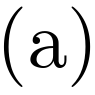
\includegraphics{figures/(a).png}\end{minipage}%
%
\begin{minipage}{0.01\linewidth}
~\end{minipage}%
%
\begin{minipage}{0.45\linewidth}
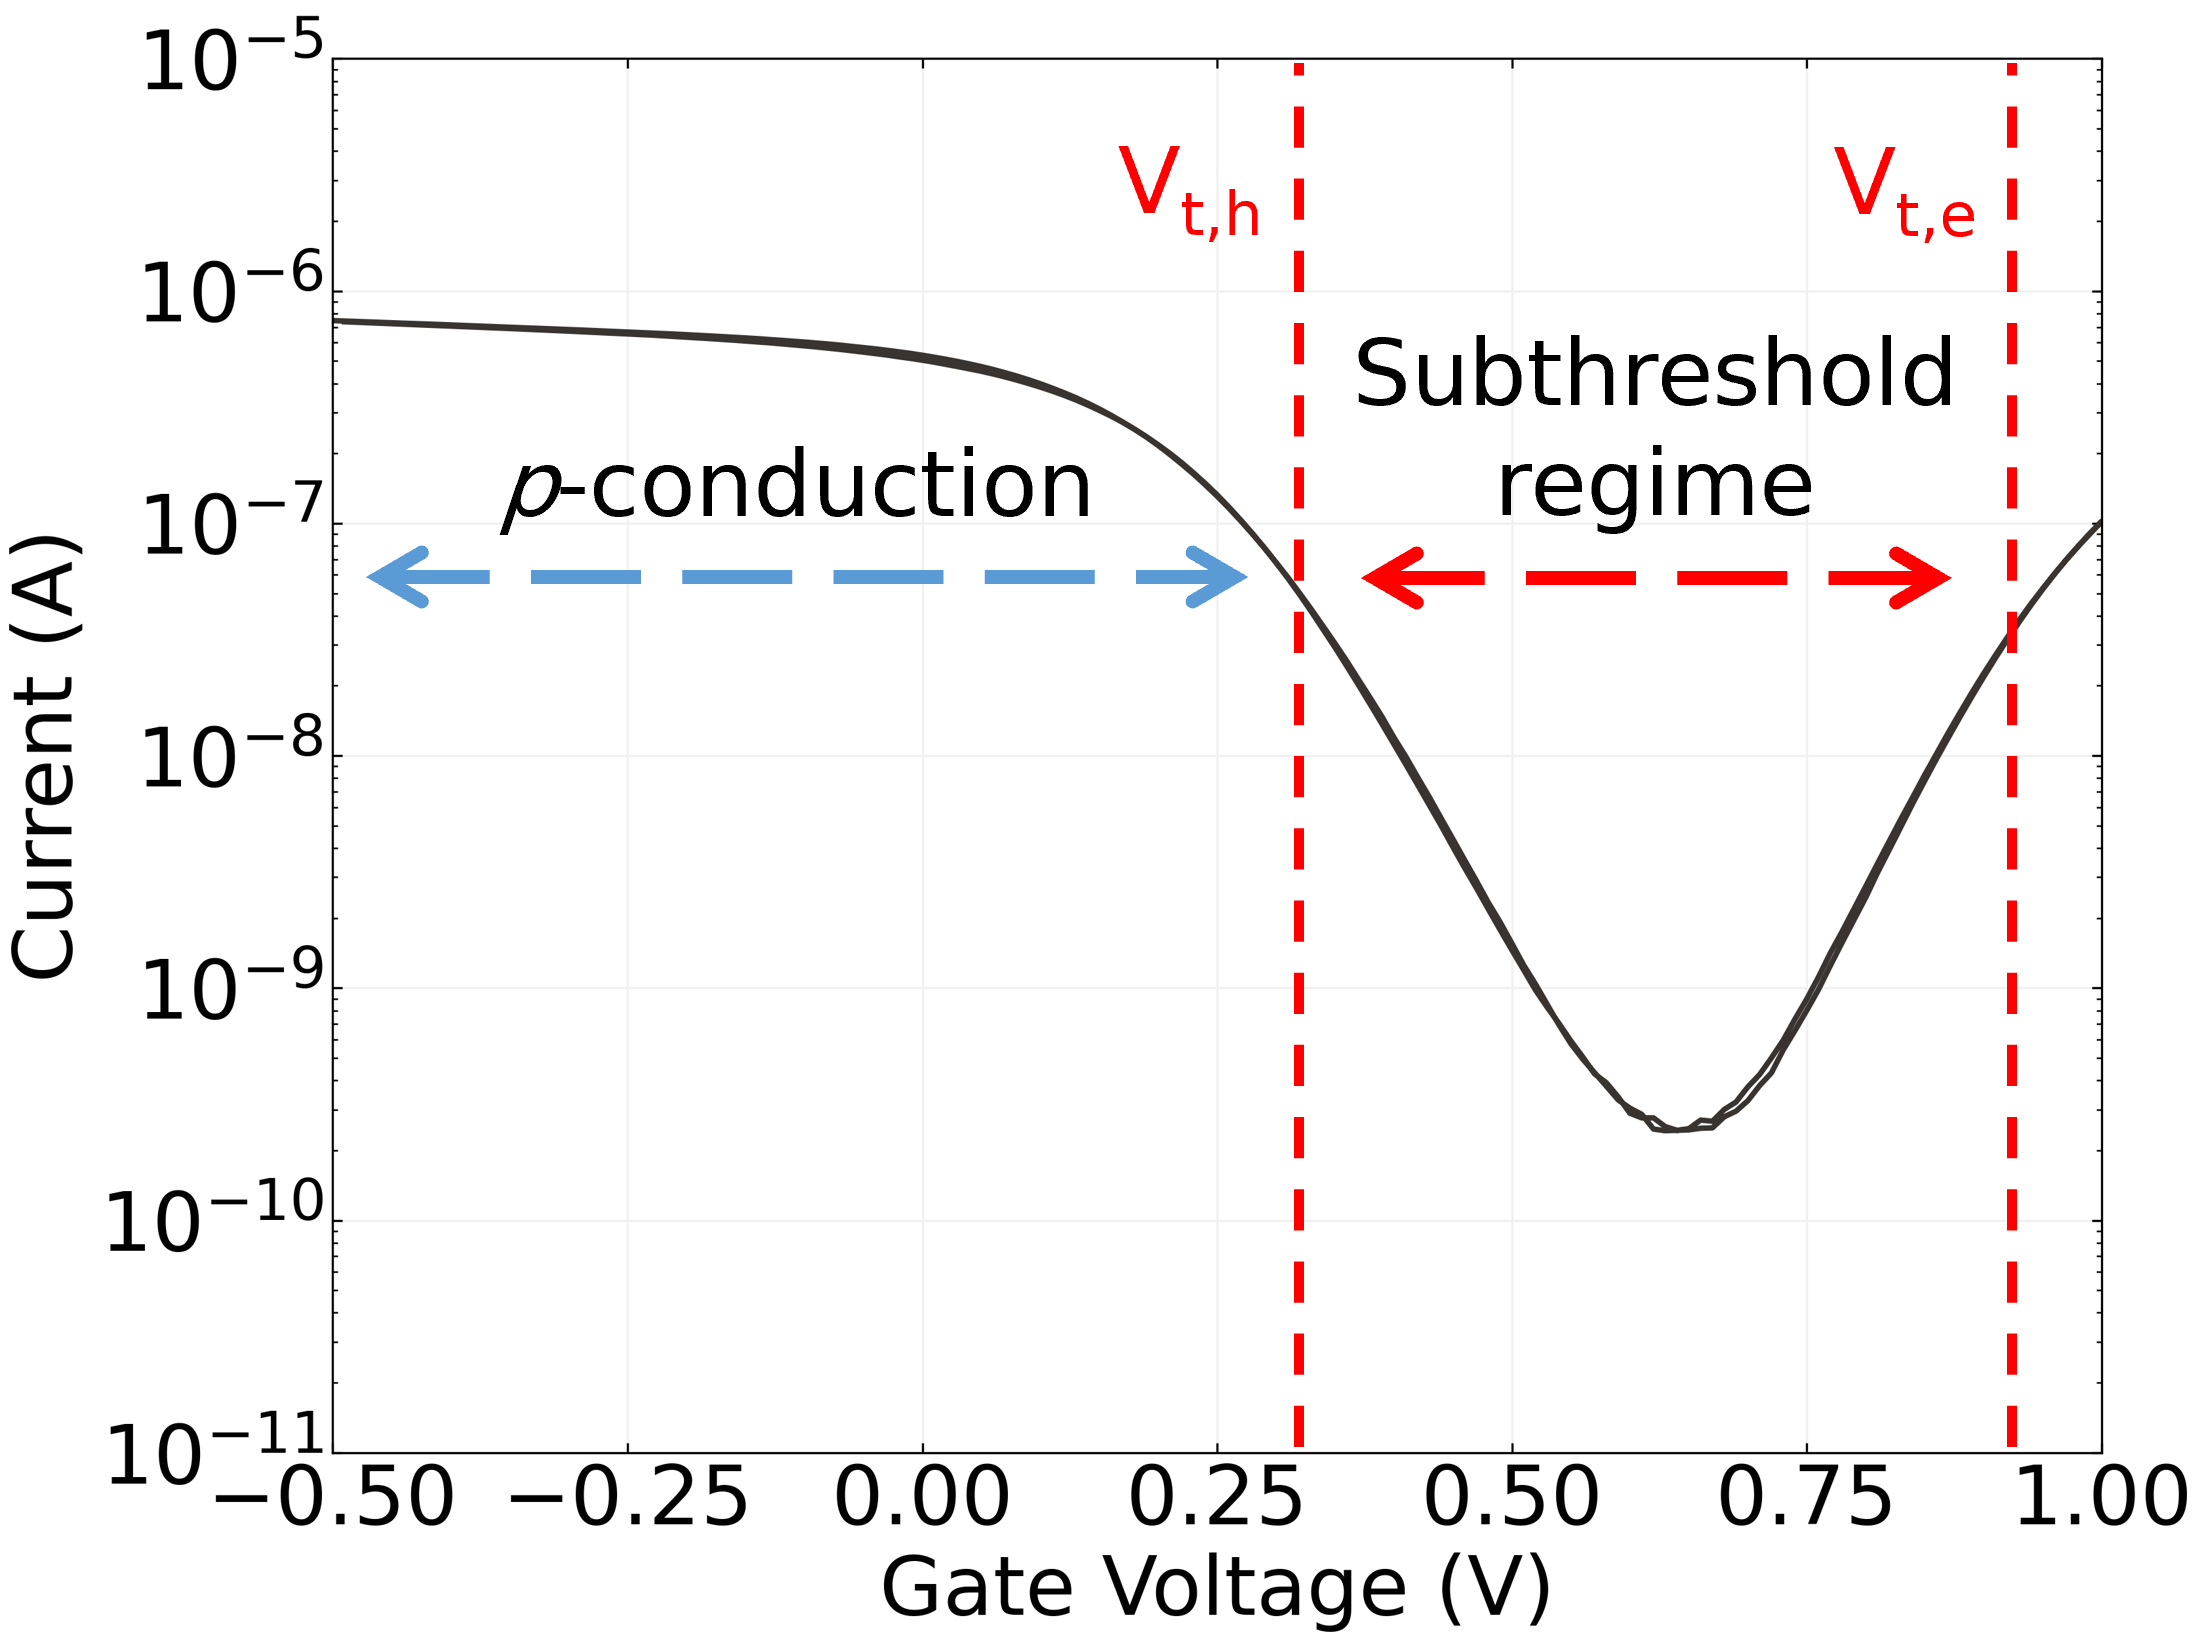
\includegraphics{figures/ch2/CNT_transfer_1.png}\end{minipage}%
%
\begin{minipage}{0.01\linewidth}
~\end{minipage}%
%
\begin{minipage}{0.03\linewidth}
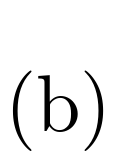
\includegraphics{figures/(b).png}\end{minipage}%
%
\begin{minipage}{0.01\linewidth}
~\end{minipage}%
%
\begin{minipage}{0.45\linewidth}
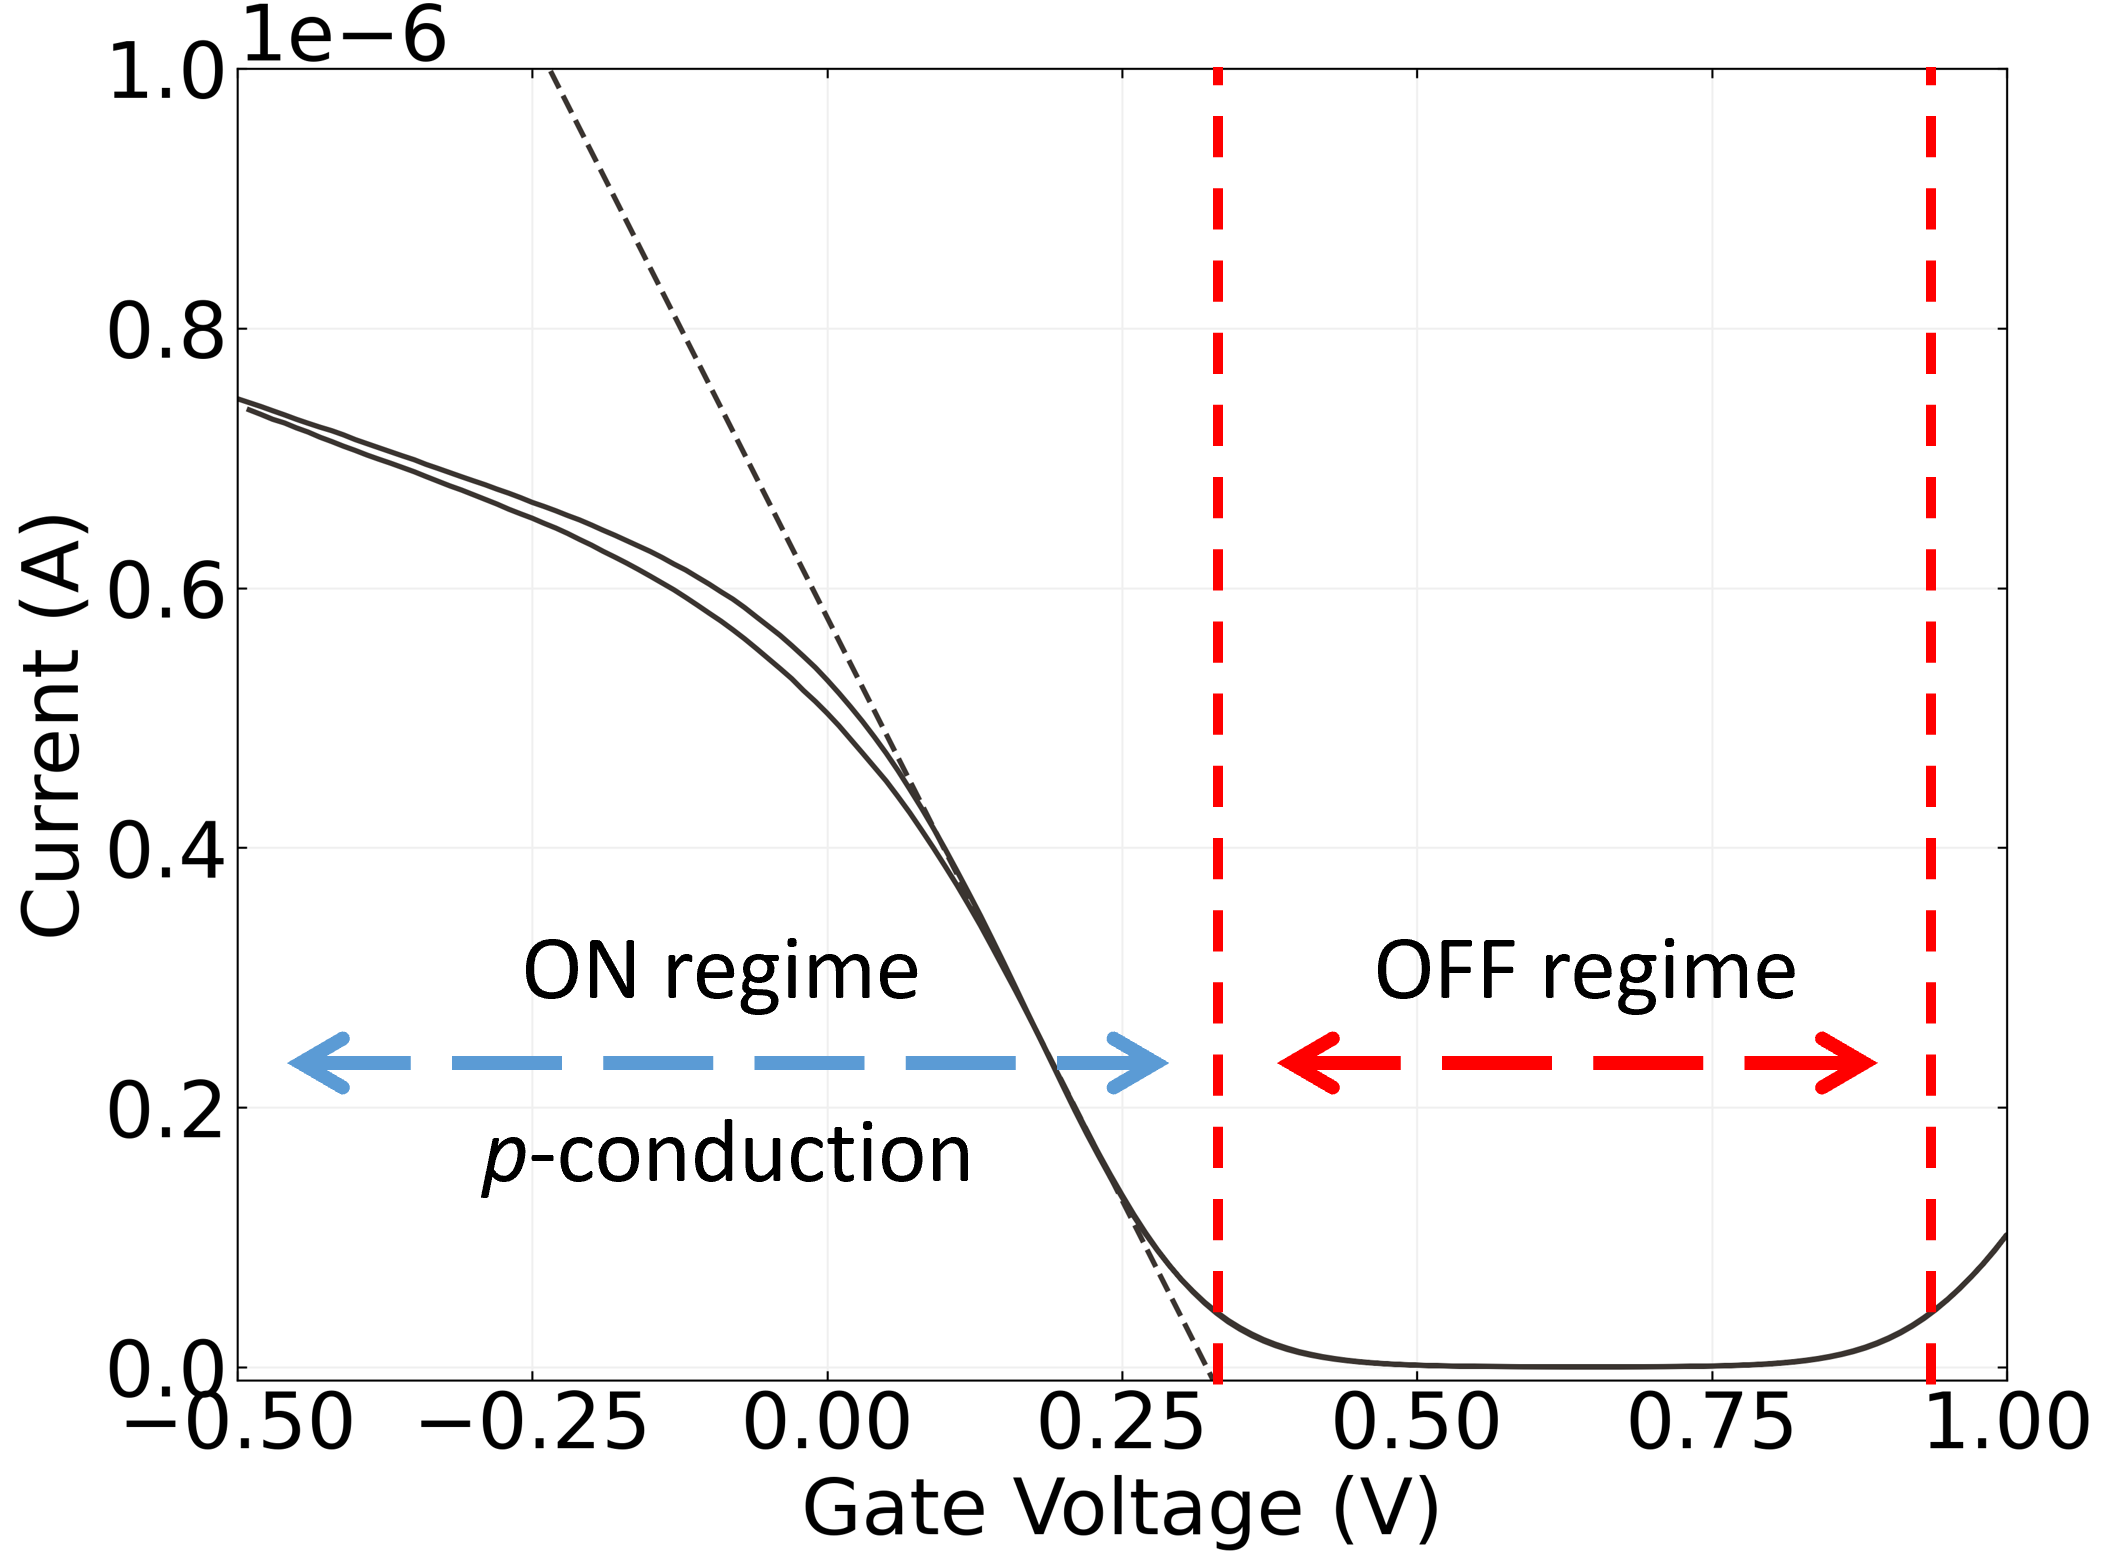
\includegraphics{figures/ch2/CNT_transfer_2.png}\end{minipage}%
%
\begin{minipage}{0.01\linewidth}
~\end{minipage}%

\caption{\label{fig-CNT-characteristics}Liquid-gated transfer
characteristics of a single carbon nanotube network field-effect
transistor channel, using a logarithmic scale in (a) and using a linear
scale in (b) to emphasise different features of the same dataset. The
subthreshold slope is shown with a black dotted line, while the
threshold voltages are shown with red dotted lines. The ON and OFF
regimes are also indicated on both figures. \(V_{ds}\) = 100 mV was
placed across the channel.}

\end{figure}%

The threshold voltage \(V_t\) of a unipolar transistor is equal to the
gate voltage required to prevent the flow of charge carriers across the
channel, often referred to as turning the device off {[}@Petti2016;
@Shkodra2021{]}. In ambipolar devices, two separate threshold voltages
exist for each type of charge carrier, \(V_{t,h}\) and \(V_{t,e}\),
which are shown in Figure~\ref{fig-CNT-characteristics} on both a linear
(a) and logarithmic (b) scale. In the region between these gate
voltages, known as the subthreshold regime, both holes and electrons
flow through the channel {[}@Avouris2007; @Reiner-Rozman2015{]}. If
percolating pathways consisting entirely of m-CNTs are present,
\(I_{off}\) flows through these pathways, as conduction through metallic
nanotubes is largely unaffected by changes in \(V_g\) {[}@Fuhrer2000;
@Topinka2009{]}. If there are no unblocked m-CNT pathways, \(I_{off}\)
is entirely due to Schottky barrier tunnelling {[}@Avouris2007{]}.
\(V_t\) can be estimated by extrapolating the trendline of the linear
region of the transfer characteristics to the \(V_g\) axis. The
intercept is approximately equal to the threshold voltage when
\(V_{ds}\) is close to zero, as shown in
Figure~\ref{fig-CNT-characteristics} (b) {[}@Sze2006; @Petti2016;
@Li2023{]}. This is only a rough estimate of the actual device \(V_t\),
but is sufficient when comparing the gating behaviour of different
devices {[}@Li2023{]}.

\begin{figure}

\centering{

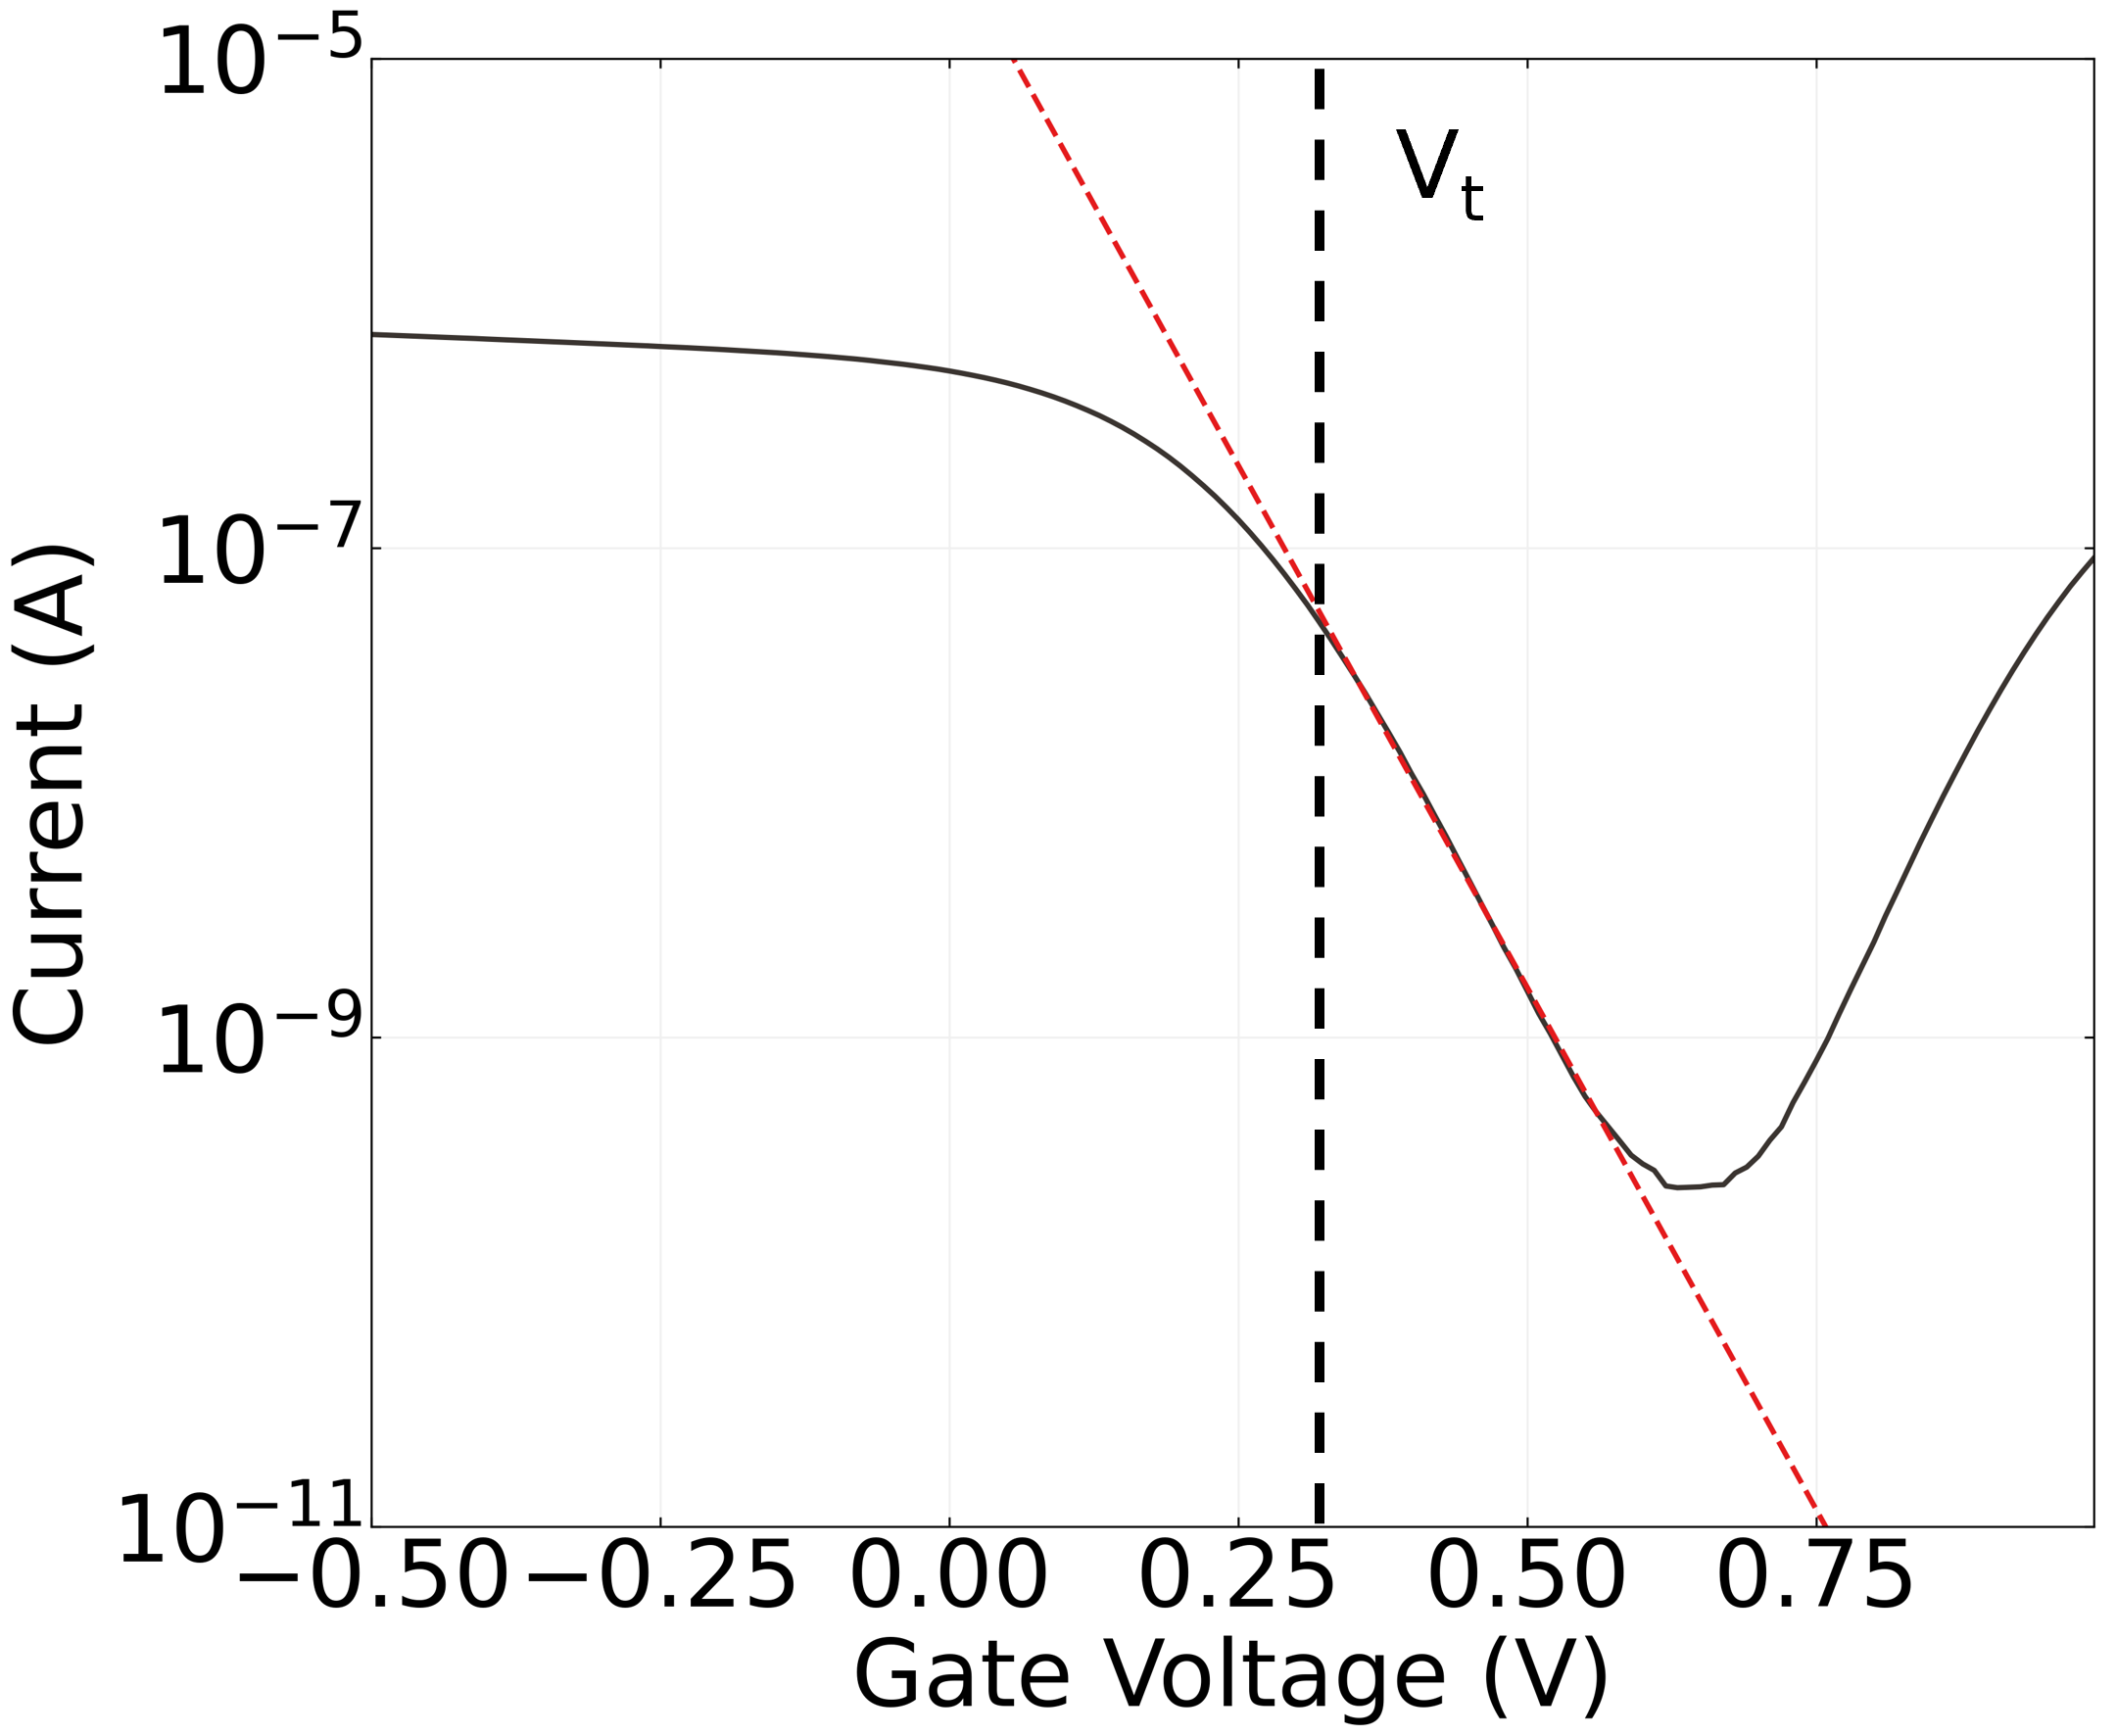
\includegraphics[width=0.45\textwidth,height=\textheight]{figures/ch2/NTQ31C5ch1subthreshold_slope_alt.png}

}

\caption{\label{fig-subthreshold-slope}A carbon nanotube network
transfer sweep with \(V_{ds}\) = 100 mV on a logarithmic scale.
Threshold voltage is shown with a black dotted line, while subthreshold
slope is shown with a red dotted line.}

\end{figure}%

The subthreshold slope
\(S = d\textrm{log}_{10}(I_{d})/dV_g|_{\textrm{max}}\) is a measure of
how rapidly a transistor approaches the minimum current \(I_{off}\). The
subthreshold slope is often referred to using its reciprocal value, the
subthreshold swing, which is equivalent to the change in \(V_g\)
required to change \(I_d\) by one order of magnitude. This figure of
merit is strongly related to the gate capacitance of the device. As the
slope exponentially approaches the off current in the subthreshold
regime, it can be fitted with a linear trendline on a logarithimic
scale. {[}@Sze2006; @Petti2016{]}. A linear trendline fitted to the
logarithm of the subthreshold regime is shown in
Figure~\ref{fig-subthreshold-slope}, where the gradient corresponds to
subthreshold slope. A high subthreshold slope exceeding than 10
decades/V is ideal for reduced power consumption of the working sensor
device {[}@Petti2016{]}. The subthreshold slope of the transfer sweep in
Figure~\ref{fig-subthreshold-slope} is 8 decades/V. Heller \emph{et al.}
and Gao \emph{et al.} found that sensor devices showed better
signal-to-noise ratio when gated in the subthreshold regime, as small
voltage changes in response to analyte led to exponential current
changes along the subthreshold slope {[}@Heller2009; @Gao2010{]}.

\subsubsection{Sensing}\label{sec-CNT-sensing-mechanisms}

As all atoms are at the surface of the carbon nanotube structure,
nanotubes are very sensitive to their surroundings and easily modified,
making them useful in biosensor applications {[}@Cao2009; @Yao2021;
@Shkodra2021{]}. The chirality and diameter of a carbon nanotube affects
both its coupling with the gate and its surface chemistry, which
determines the sensing mechanisms available to a single CNT. Only s-CNTs
can be electrostatically gated; m-CNTs, bent nanotubes and larger
diameter nanotubes are typically more reactive {[}@Cao2009; @Zhao2012;
@Chhikara2013; @Li2023{]}; and the nanotube chirality (\(n,m\)) can
determine the strength of binding to DNA in a base sequence-dependent
manner {[}@Rouhi2011a{]}. Carbon nanotubes have been used for
vapour-phase sensing since 2000, when Kong \emph{et al.} found that the
resistance over a single CNT channel was modified when exposed to gas
molecules like NO\(_2\) and NH\(_3\) {[}@Kong2000{]}. Carbon nanotubes
have been used to detect the presence of analyte down to the parts per
billion level in a variety of gas sensor applications {[}@Chen2019;
@Yao2021{]}. However, in general, the specificity of such a sensor is
low, as nanotubes respond to many different analytes in a similar
manner. To enhance specificity, surface functionalisation is often
performed using either inorganic or biological materials, such as
enzymes, antibodies, aptamers and proteins {[}@Cao2009; @Shkodra2021;
@Yao2021{]}.

For carbon nanotube network transistors, sensing mechanisms include
electrostatic gating, charge transfer, Schottky barrier modulation,
modulation of channel capacitance relative to the electrolyte and charge
scattering. Response mechanisms may take place at the gate, the
junctions between channel and contact, or at the semiconductor channel
{[}@Heller2008; @Battie2011; @Boyd2014; @Tran2016; @Li2023{]}.
Modification of the channel-metal Schottky barrier can dominate sensing
activity, and this can complicate the identification of mechanisms
underlying the sensing behaviour {[}@Cao2009; @Boyd2014;
@Schroeder2019{]}. The encapsulation layer shown in
Figure~\ref{fig-gating-schematics} is added to separate the electrodes
from the channel-metal junction and prevent these responses
{[}@Heller2008; @Shkodra2021{]}. In an encapsulated device, the
predominant sensing mechanism is either charge transfer from the analyte
to channel {[}@Allen2007; @Battie2011{]} or electrostatic gating
{[}@Heller2008{]}. The charge transfer mechanism involves direct
addition of charge carriers to the channel, while the gating mechanism
results from a nearby charge inducing an opposite polarity charge in the
channel. Both changes alter the relationship between \(V_g\) and \(I_d\)
and shift the carrier threshold voltage(s) {[}@Tran2016; @Shkodra2021;
@Li2023{]}. Modulation of Schottky and other potential barriers present
in the network may also make a significant contribution to sensing
responses, especially when a network is close to its percolation
threshold {[}@Boyd2014; @Murugathas2019{]}.

\subsection{Summary}\label{summary}

Graphene and carbon nanotube network field-effect transistors are both
ideal as the transducer element in sensing applications due to their
excellent electrical properties and high sensitivity. These thin-film
FETs can be used as sensor platforms in either a back-gated or
liquid-gated configuration, where the liquid-gated configuration is used
in aqueous sensing applications. A key attribute of the liquid-gated
configuration is Debye length, which must be optimised for maximum
transistor sensitivity. Important device parameters of the graphene and
carbon nanotube network FETs include transconductance, on-off ratio,
gate leakage currents, current hysteresis, threshold voltage and
sub-threshold slope. The voltage corresponding to the Dirac point (or
points) of graphene is another important figure of merit for graphene
field-effect transistors. Various attributes of the morphology of
graphene and carbon nanotube networks contribute to the unique
electrical and sensing properties exhibited by these transistors,
including graphene folds and junctions between nanotubes of different
chirality. The use of these transducers in past odorant receptor
biosensor applications is discussed in \textbf{?@sec-iOR-sensors}, while
fabrication of the transducers used here is detailed in
\textbf{?@sec-fabrication}.




\end{document}
